\documentclass[oneside, a4paper,12pt]{ltxdoc}
\usepackage{geometry}
\usepackage{hyperref}
\usepackage{phd}
\tcbuselibrary{documentation}
 
\makeatletter\makeatother

%to break urls
\expandafter\def\expandafter\UrlBreaks\expandafter{\UrlBreaks%  save the current one
  \do\a\do\b\do\c\do\d\do\e\do\f\do\g\do\h\do\i\do\j%
  \do\k\do\l\do\m\do\n\do\o\do\p\do\q\do\r\do\s\do\t%
  \do\u\do\v\do\w\do\x\do\y\do\z\do\A\do\B\do\C\do\D%
  \do\E\do\F\do\G\do\H\do\I\do\J\do\K\do\L\do\M\do\N%
  \do\O\do\P\do\Q\do\R\do\S\do\T\do\U\do\V\do\W\do\X%
  \do\Y\do\Z}
\Urlmuskip = 2mu plus 1mu 
\makeatletter
\cxset{plain sections/.style={
 chapter name = CHAPTER,
 chapter toc = true,
 chapter color= thegray,
 chapter opening = right, 
 chapter numbering = arabic,
 chapter font-family= sffamily,
 chapter font-weight= bold,
 chapter font-size= LARGE,
 chapter before={\thinrule\vspace*{20pt}\par\hfill\hfill},
 chapter after={\vskip0pt\par},
 chapter spaceout = soul,
 number font-size= Large,
 number font-family= rmfamily,
 number font-weight= bfseries,
 number color=thegray,
 number before=\vspace*{5pt}\hfill\hfill,
 number dot=.,
 number after={\hspace*{7pt}\par},
 title beforeskip={\vspace*{10pt}},
 title afterskip={\vspace*{50pt}\par},
 title before={\hfill\hfill\raggedleft},
 title after={\par\thinrule},
 title font-family=\sffamily,
 title font-color= teal,
 title font-weight=\bfseries,
 title font-family=\sffamily,
 title font-size= Large,
 title font-shape= upshape,
 title spaceout= none,
 title beforeskip={\vspace*{10pt}},
 title afterskip={\vspace*{50pt}\par},
 title before={\hfill\hfill\raggedleft},
%
% numbers
% number font-family=\sffamily,
% number font-weight=\bfseries,
 number color=thelightgray,
 number before=\par\vspace*{5pt}\hfill\hfill,
 number dot=,
 number after={\hspace*{7pt}\par},
 number position=rightname,
 section color= thered,     
 section beforeskip=15pt,
 section afterskip=15pt,
 section indent=0pt,
 section font-family= sffamily,
 section font-size= LARGE,
 section font-weight= bfseries,
 section font-shape=,
 section align= centering,
 section numbering prefix =,%use \thechapter. for books or add as option
 section numbering= arabic,
 section spaceout=none,
 section number after=ooo,
 subsection color= thered,
       subsection beforeskip=10pt,
       subsection afterskip=10pt,
       subsection indent=0pt,
       subsection font-family= rmfamily,
       subsection font-size= large,
       subsection font-weight= bold,
       subsection font-shape= upshape,
       subsection align= centering,
       subsection numbering prefix=\thesection.,%\S\hairsp,%add . 
       subsection numbering custom =\@arabic\c@subsection,% \two@digits{\@arabic\c@subsection},%
       subsubsection color= gray,
       subsubsection beforeskip=5pt plus3pt minus 2pt,
       subsubsection afterskip=5pt,
       subsubsection indent=0pt,
       subsubsection font-family= rmfamily,
       subsubsection font-size= normalfont,
       subsubsection font-weight= bold,
       subsubsection font-shape= itshape,
       subsubsection align= centering,
       subsubsection numbering prefix =\thesubsection.\@arabic\c@subsubsection,
       subsubsection numbering custom =, %\two@digits{\@arabic\c@subsubsection},
       subsubsection number after =, 
%
       paragraph color= thegrey,
       paragraph beforeskip=,
       paragraph afterskip=-0.5em,
       paragraph indent=0pt,
       paragraph font-family= rmfamily,
       paragraph font-size= large,
       paragraph font-weight= bfseries,
       paragraph font-shape=,
       paragraph align= centering,
       paragraph number after = 0pt,
       paragraph numbering=numeric,
       subparagraph color= thered,
       subparagraph beforeskip=0pt,
       subparagraph afterskip=-.5em,
       subparagraph indent=0pt,
       subparagraph font-family= sffamily,
       subparagraph font-size= large,
       subparagraph font-weight= normalfont,
       subparagraph font-shape= slshape,
       subparagraph align= RaggedRight,
       subparagraph number after =, % can affect all needs checking
       %subsubsection numbering prefix=\S\hairsp\thesection,%add . here if need be
       subparagraph numbering=none,
}
}
\cxset{plain sections}
\cxset{style13/.style={
 name= {\protect\pan अमुकग्रन्थे},
 chapter spaceout = none,
 numbering=arabic,
 number font-size= HUGE,
 number font-family= sffamily,
 number font-weight= bfseries,
 number color= gray!50,
 number before=\par\vspace*{5pt}\hfill\hfill,
 number dot=,
 number after={\hspace*{7pt}\par},
 number position=rightname,
 chapter font-family= sffamily,
 chapter font-weight= bold,
 chapter font-size= LARGE,
 chapter before={\tikzrule\vspace*{20pt}\par\hfill\hfill},
 chapter color= black!50,
 title beforeskip={\vspace*{10pt}},
 title afterskip={\vspace*{50pt}\par},
 title before={\hfill\hfill\raggedleft},
 chapter rule color=teal,
 title after=\par\tikzrule,
 title font-family= sffamily,
 title font-color= teal,
 title font-weight= bfseries,
 title font-size= huge,
 section indent=-1em,
 section align= left,
 section numbering= arabic,
 section indent=0pt,
 section beforeskip=0pt,
 section afterskip= 10pt,
 section color=teal,
 subsection align= ,
 subsection font-family= sffamily,
 subsection font-weight= bfseries,
 subsection color = teal,
 subsection font-size= large,
 subsection font-shape=,
 subparagraph number after=,
 subsubsection align=,
}
}
\cxset{style13}

\renewparagraph
\renewsection
\renewsubsection
\renewsubparagraph
\renewsubsubsection

\makeatother

\definecolor{niagra}{rgb}{0.7,0.027,0.22}
\definecolor{tiber}{rgb}{0.0039,0.09,0.27}

\cxset{%
 chapter color=tiber,
 title font-color=tiber,
 section afterindent = false, 
 section color= tiber,     
 section beforeskip=15pt,
 section afterskip=15pt,
 section indent=-3cm,
 section font-family= sffamily,
 section font-size= LARGE,
 section font-weight= bfseries,
 section font-shape=,
 section align= left,
 section numbering prefix =\thechapter.,
 section numbering= arabic,
 section spaceout=soul,
  section numbering suffix=,
 }
\cxset{title font-color=tiber,
chapter rule color=thegray}
\makeatletter
\begingroup \catcode `|=0 \catcode `[= 1
\catcode`]=2 \catcode `\{=12 \catcode `\}=12
\catcode`\\=12 |gdef|@xsmallverbatim#1\end{smallverbatim}[#1|end[smallverbatim]]
|gdef|@sxsmallverbatim#1\end{smallverbatim*}[#1|end[smallverbatim*]]
|endgroup
\def\@smallverbatim{\trivlist \item\relax
  \if@minipage\else\vskip\parskip\fi
  \leftskip\@totalleftmargin\rightskip\z@skip
  \parindent\z@\parfillskip\@flushglue\parskip\z@skip
  \@@par
  \@tempswafalse
  \def\par{%
    \if@tempswa
      \leavevmode \null \@@par\penalty\interlinepenalty
    \else
      \@tempswatrue
      \ifhmode\@@par\penalty\interlinepenalty\fi
    \fi}%
  \let\do\@makeother \dospecials
  \obeylines \smallverbatim@font \@noligs
  \hyphenchar\font\m@ne
  \everypar \expandafter{\the\everypar \unpenalty}%
}
\def\smallverbatim{\@smallverbatim \frenchspacing\@vobeyspaces \@xsmallverbatim}
\def\endsmallverbatim{\if@newlist \leavevmode\fi\endtrivlist}

\def\smallverbatim@font{\normalfont\smallverbatimsize\ttfamily}


\def\@sect#1#2#3#4#5#6[#7]#8{%
  \ifnum #2>\c@secnumdepth
   \let\@svsec\@empty
  \else
  \refstepcounter{#1}%
  \protected@edef\@svsec{\@seccntformat{#1}\relax}%
 \fi
 \@tempskipa #5\relax
 \ifdim \@tempskipa>\z@
 \begingroup
#6{%
 \@hangfrom{\hskip #3\relax\@svsec}%
 \interlinepenalty \@M #8\@@par}%
 \endgroup
 \csname #1mark\endcsname{#7...}%
 \addcontentsline{toc}{#1}{%
 \ifnum #2>\c@secnumdepth \else
   \protect\numberline{\csname the#1\endcsname}%
 \fi
 #7}%
 \else
 \def\@svsechd{%
 #6{\hskip #3\relax
  \@svsec #8}%
 \csname #1mark\endcsname{#7}%
 \addcontentsline{toc}{#1}{%
 \ifnum #2>\c@secnumdepth \else
      \protect\numberline{\csname the#1\endcsname}%
 \fi
 #7}}%
 \fi 
 \@xsect{#5}}
 
  
\cxset{geometry/.is choice,
          geometry/elements/.code = \geometry{ heightrounded,
          includeheadfoot=false,
          textwidth=      251pt,
          textheight=     502pt,
          paperwidth=     374pt,
          paperheight=    648pt,
          vmarginratio=   1:2,
          marginparwidth= 60pt,
          marginparsep=   18pt,
          outer=          90pt}}   
          
\cxset{geometry/aureo/.code=\geometry{ heightrounded,
         includeheadfoot=true, 
         textwidth=      120mm,
         textheight=     194mm,
         paperwidth=     17cm,
         paperheight=    24cm,
         marginratio=    2:3,
         marginparwidth= 62pt,
         marginparsep=   10pt}}            
    
\cxset{geometry/compact aureo/.code= \geometry{
    heightrounded,
    includeheadfoot=false,
    textheight=     175mm,
    textwidth=      108mm,
    paperwidth=     140mm,
    paperheight=    210mm,
    marginratio=    1:1,
    marginparwidth= 11mm,
    marginparsep=   7pt}
}    

\cxset{geometry/super compact/.code= 
\geometry{
    heightrounded,
    includeheadfoot=false,
    textheight=     175mm,
    textwidth=      108mm,
    paperwidth=     140mm,
    paperheight=    210mm,
    marginratio=    1:1,
    marginparwidth= 11mm,
    marginparsep=   7pt}    
}
 
\cxset{geometry/standard/.code=                   
 \geometry{%standard
    heightrounded,
    a4paper,
    includeheadfoot=true,
    textwidth=      110mm,
    textheight=     220mm,
    marginratio=    1:2,
    marginparwidth= 30mm,
    marginparsep=   12pt}}   
    
\cxset{geometry/periodical/.code=                  
 \geometry{%periodical
    heightrounded,
    includeheadfoot=false,
    textheight=     165mm,
    textwidth=      110mm,
    paperwidth=     170mm,
    paperheight=    240mm,
    marginratio=    2:3,
    marginparwidth= 26mm,
    marginparsep=   10pt}}   
    
\cxset{geometry/periodical aureo/.code= \geometry{%periodical aureo
    heightrounded,
    includeheadfoot=true,
    textwidth=      120mm,
    textheight=     194mm,
    paperwidth=     17cm,
    paperheight=    24cm,
    marginratio=    2:3,
    marginparwidth= 62pt,
    marginparsep=   10pt}}
    
\cxset{geometry/tufte a4paper/.code=    
      \geometry{a4paper,heightrounded,
        left=24.8mm,top=27.4mm,headsep=2\baselineskip,textwidth=107mm,
       marginparsep=8.2mm,marginparwidth=49.4mm,
       textheight=661.5pt,headheight=\baselineskip,
       }}  %error on asymetr
       
\cxset{geometry/tufte letterpaper/.code=\geometry{%  
        heightrounded,     
        letterpaper,left=1in,top=1in,headsep=2\baselineskip,textwidth=26pc,marginparsep=2pc,
       marginparwidth=12pc,textheight=594pt,
       headheight=\baselineskip\relax,reversemp=true,
       twoside=false
       }}         
%  

\cxset{newgeometry/.is choice,
        newgeometry/tufte letterpaper/.code=\newgeometry{%  
        heightrounded,     
        letterpaper,
        left=1in,
        top=1in,
        headsep=2\baselineskip,textwidth=26pc,marginparsep=2pc,
       marginparwidth=12pc,textheight=594pt,
       headheight=\baselineskip\relax,
       reversemp=false,
       twoside=true}}  



%\cxset{geometry=standard}    

\makeatother
\cxset{geometry=standard}    
\begin{document}

%               \makeatletter
%              \@twosidetrue\@mparswitchfalse

                    
%\tableofcontents
\cxset{mainmatter numbering=arabic}
\def\innermarginname{Inner}
\mainmatter

%\lipsum[1-10]
%
%\cxset{geometry units=mm}
%\pagestyle{grid}

\chapter{Margin Material}

\section{Introduction}

Since the beginning of writing margins were always used to add notes and other marginal material such as citations, notes and even figures. The \pkgname{marginnote} developed by \citeyearpar{marginnote} does not float the marginal
notes and for a good reason, as most of the time they end up in the wrong place in any case. This chapter describes
the usage of marginpar and not the technicalities of the definitions. The definitions are described in the |float.dtx| in 
\nameref{ltx:marginalnotes}

\section{How to Switch Margin paragraphs}

Marginal notes use the same mechanism as floats to communicate with the \cmd{\output} routine.
Marginal notes are distinguished from floats by having a negative placement specification. [372-373] The \CMDI{\marginpar}\oarg{left text}\marg{right text} generates a marginal note in parbox, using either the left 
text or the right text, depending on the placement. It default to righttext=lefttext. 

\begin{figure}
\includegraphics[width=\textwidth]{marginpar-01}
\end{figure}

Most designers appear to prefer to use only the one side of the page, when margin materials form part of the design of the book, such as the tufte-class. 

Marginal notes are normally put on the outside of the page if the switch \CMDI{\@mparswitch} is true, and on the right if |@mparswitch=false|. The command \CMDI{\reversemarginpar} reverses the side where they are put. \CMDI{\normalmarginpar} undoes |\reversemarginpar|. These commands have no effect in two-colum output.


\begin{figure}
\includegraphics[width=\textwidth]{marginpar-02}
\end{figure}


\lipsum
\makeatletter
\newenvironment{adjustmargins}[2]{%
 \begin{list}{}{%
 \topsep\z@%
 \listparindent\parindent%
 \parsep\parskip%
 \checkoddpage
 \ifoddpage % odd numbered page
 \@ifmtarg{#1}{\setlength{\leftmargin}{\z@}}%
 {\setlength{\leftmargin}{#1}}%
 \@ifmtarg{#2}{\setlength{\rightmargin}{\z@}}%
 {\setlength{\rightmargin}{#2}}%
 \else % even numbered page
 \@ifmtarg{#2}{\setlength{\leftmargin}{\z@}}%
 {\setlength{\leftmargin}{#2}}%
 \@ifmtarg{#1}{\setlength{\rightmargin}{\z@}}%
 {\setlength{\rightmargin}{#1}}%
\fi
}
\item[]}{\end{list}}

\makeatother
\chapter{Pages}

\parindent1em
The page is the main element in a book and its geometry and layout has been studied extensively by typographers. In this chapter we outline the typographical tradition, methods to specify layouts using \latex and associated issues, such as adjusting margins within a page.

Bringhurst notes that ``much typography is based, for the sake of economy on standard industrial sizes, from $35\times45$ inch press sheets to $3 1/2$ x 2 inch conventional business cards. Some formats as the booklets that accompany compact discs, are condemned to especially rigid restrictions of size.  If you are writing a thesis or are bound by business rules to use a specific size, there is not much that you can do in terms of page layouts, but if you have the opportunity and necessity of selecting the dimensions of the page you have a great opportunity to enhance the page layout of your book.

\section{Selecting a page size}

How do you select a size? History, natural science, geometry and mathematics
are all relevant to typography in this regard -- and can all be counted on for aid.

\begin{figure}[ht]
\centering
\includegraphics[width=0.5\textwidth]{./images/preparing-paper.jpg}
\caption{Getting paper prepared for printing \citep{moxon}.}
\end{figure}

Originally, paper sizes were determined by the moulds the paper was
made in and the use the result was put to. While many hundreds of variations have occurred throughout the centuries, in the main there have seldom been more than six categories of sizes in use since the fourteenth century. These have often come down to us bearing the names of the figures featured in the paper's watermarks, such as foolscap,
elephant, pot, and crown. To enable the creation of smaller sizes from
existing larger sizes, the sheets have since the Middle Ages been proportioned
with their sides in the ratio of \(1:\sqrt{2}\). For example, quarto (4to,
formerly 4to) and octavo (8vo, formerly 8vo) sizes are obtained by cutting
or folding standard sizes four and eight times respectively.
Former British paper dimensions still used the old sizes before decimalized
versions replaced them; US dimensions still retain most of these
(untrimmed) paper sizes, in inches. Both are still encountered in specialist and bibliographic work, and in reproducing earlier or foreign formats:



Typographers derive proportions that naturally occur in nature, and pages that embody
them recur in manuscripts and books from Rennaissance Europe, Tang and Song dynasty
China, early Egypt and ancient Rome.  
These numbers are $\pi=$3.14159\ldots , which is the circumference of a circle whose diameter
is one; $\sqrt{2}=$1.41421\ldots , which is the diagonal of a unit square; 
$e=2.71828$  \ldots ,which is the base of the natural logarithms; and $\phi=1.61803$ \ldots ,a number which is discussed later on. Certain of these proportions appear in he structure of the human body; other appear in musical scales. Indeed, one of the simplest of all systems of 
page proportions is based on the familiar intervals of the diatonic scale. Pages that
embody these basic musical proportions have been in common use in Europe for more than a thousand year.

\begin{figure}[hb]
\cxset{spread xsteps=9,
       spread scale=0.20,
       spread width=0.5\textwidth}
\centering
\drawcanons
\end{figure}


\begin{figure}
  \includegraphics[width=0.5\linewidth]{./graphics/A-sizes.png}
  \caption{\large When a sheet whose proportions are $1$:$\surd{2}$ is folded in half, the result is a sheet half as large but with \emph{the same proportions}. Standard paper sizes on this principle have been in use in Germany since the early 1920s. The basis of this system is teh A0 sheet, which has an are of 1 m$^2$. Yes because it is \textit{reciprocal with nothing but itself}, the ISO page in isolation is the least musical of all the major page shapes. It needs a textblock of another shape or contrast.}
   \label{fig:marginfig1}
\end{figure}

The advantages of basing a paper size upon an aspect ratio of $\surd{2}$ were already noted in 1786 by the German scientist Georg Christoph Lichtenberg, in a letter to Johann Beckmann[2]. The formats that became A2, A3, B3, B4 and B5 were developed in France, and published in 1798 during the French Revolution, but were subsequently forgotten.[3]

Early in the twentieth century, Dr Walter Porstmann turned Lichtenberg's idea into a proper system of different paper sizes. Porstmann's system was introduced as a DIN standard (DIN 476) in Germany in 1922, replacing a vast variety of other paper formats. Even today the paper sizes are called "DIN Ax" in everyday use in Germany.

The main advantage of this system is its scaling: if a sheet with an aspect ratio of $\surd{2}$ is divided into two equal halves parallel to its shortest sides, then the halves will again have an aspect ratio of $\surd{2}$. Folded brochures of any size can be made by using sheets of the next larger size, e.g. A4 sheets are folded to make A5 brochures. The system allows scaling without compromising the aspect ratio from one size to another – as provided by office photocopiers, e.g. enlarging A4 to A3 or reducing A3 to A4. Similarly, two sheets of A4 can be scaled down and fit exactly 1 sheet without any cutoff or margins.

\cxset{try grid=false}
\thispagestyle{grid}

\drawlist

The weight of each sheet is also easy to calculate given the basis weight in grams per square metre (g/m2 or `'gsm"). Since an A0 sheet has an area of 1 m2, its weight in grams is the same as its basis weight in g/m². A standard A4 sheet made from 80 g/m² paper weighs 5g, as it is one 16th (four halvings) of an A0 page. Thus the weight, and the associated postage rate, can be easily calculated by counting the number of sheets used.

Unlike the |A4| standard paper, the origin of the dimensions of letter size paper are lost in tradition. The American Forest and Paper Association argues that the dimension originates from the days of manual paper making, and that the 11-inch length of the page is about a quarter of ``the average maximum stretch of an experienced vatman's arms".[1] However, this does not explain the width or aspect ratio. What is known is that Ronald Reagan made this the paper size for U.S. federal forms; previously, the smaller "official" size (8 in × 10½ in or 203.2 mm × 266.7 mm) was used.[1] Letter or US Letter is the most common paper size for office use in the United States and Canada. It is 8$\frac{1}{2}$ by 11 inches (exactly 215.9 mm × 279.4 mm).

\section{The Typearea}

According to Bringhurst\cite{bringhurst2005}, in typography margins must do three things. They must lock the
textblock to the page and lock the facing pages to each other through the force of their proportions. Second, they must frame the textblock
in a manner that suits its design. Third, they must protect the textblock, leaving it easy for the reader to see and convenient to handle. 

In most well designed books fifty per cent of the character and integrity of a printed page lies in its letterforms. Much of the other fifty per cent resides in its margins.

\subsection{Readability}

\section{Examples}
Folowing the nomenclature introduced in bringhurst in analyzing the examples on the following pages, 
these symbols are used:

%% Align at the = sign 
\begin{table}[htbp]
\begin{tabular}{l l @{ = } p{6cm}}
\textit{Proportions:}      &P  &  page proportion $h/w$\\
~                      &T &  textblock proportion: $d/m$\\
\textit{Page size:}         &w &  width of page (trim-size)\\
~                      &h  & height of page (trim-size)\\
\textit{Textblock:}           &m & measure (width of primary textblock)\\
~                      &d  & depth of primary textblock (excluding running heads, folios etc)\\                      
~                      &$\lambda$ & line height (type size plus added lead)\\
~                      &$n$ & secondary measure (width of secondary column)\\
~                      &$c$  & column width, where there are even multiple columns\\
\textit{Margins}  &$s$  & spine margin (back margin)\\
~                      &$t$   & top margin (header margin)\\
                        &$e$  & fore-edge (front margin)\\
                        &$f$   & foot margin\\
                        &$g$  & internal gutter (on a multiple-column page)\\
\end{tabular}
\caption{Symbols used to demonstrate various ratios in books}
\end{table}
\medskip

\begin{figure}
  \includegraphics[width=\linewidth]{./graphics/page.png}
  \caption{Page nomenclature}
   \label{fig:marginfig1}
\end{figure}

More variables are necessary to specify all the variables handled by a \latex\
page. For the time being the examples refer to dimensions from historical works
in typography and should sufffice.

\subsection{Hypneroto}

\begin{figure}[htbp]
\centering
  \includegraphics[width=0.67\linewidth]{./graphics/hypneroto.jpg}
\caption{The work is lauded for the originality of its
design. Several sequential double page
illustrations add a visual dimension to the
progression of the narrative, and act like an
early form of the strip cartoon. There is an
obsession with movement throughout which is driven
on by the illustrations, resulting in the
impression of bodies moving from one page to the
next. Other typographical innovations include
playing with the traditional layout of the text;
in the opening shown here, for example, the pages
are shaped in the form of goblets. The dimensions
of the text are: $P=1.5[2:3]$; T=1.7 (tall pentagon);
Margins: s=t=w/9; e=2 s. The text is a fantasy
novel, Francesco Colonna's Hypnerotomachia
Poliphili, set in a roman font cut by Francesco
Griffo. (Aldus Manutius, Venice, 1499). Original
size: $20.5 \times 31$ cm.}
\label{fig:hypneroto}
\end{figure}


%  \label{fig:layout}



The book was printed by Aldus Manutius in Venice in December 1499. The book is anonymous, but an acrostic formed by the first, elaborately decorated letter in each chapter in the original Italian reads \textsc{\small POLIAM FRATER FRANCISCVS COLVMNA PERAMAVIT}, \enquote{Brother Francesco Colonna has dearly loved Polia.} However, the book has also been attributed to Leon Battista Alberti by several scholars, and earlier, to Lorenzo de Medici. The latest contribution in this respect was the attribution to Aldus Manutius, and arguably, a Francesco Colonna, a wealthy Roman Governor. The author of the illustrations is even less certain, but contemporary opinion gives the work to Benedetto Bordone.




\section{Temporarily changing the text width}

\index{pagewidth>change temporarily}


Margins in a page can be changed temporarily by adjusting, the lengths of \cmd{leftmargin} and \cmd{rightmargin}. The |memoir| class provides an environment |adjustwidth| see page 422 (based on This code is based on the \cmd{chngpage} package.) for doing so and the |tufte-book| class provides an environment |fullwidth|. The following code is an adaptation of that found in the |memoir| class.


\begin{teXX}
\begin{adjustmargins}{left}{right} 
\end{teXX}


adds the given lengths to the left and
right hand margins. A positive value will shorten the text and a negative value
will widen it. The starred version of the environment will cause the margin changes to switch between odd and even pages. 



\eject
\newgeometry{left=10mm,right=10mm,bottom=1.5cm,top=1cm}

\section*{The \texttt{adjustmargins} environment}
\lorem

\vfill\vfill
\begin{multicols}{2}
\lorem
\end{multicols}

\begin{adjustmargins}{0cm}{0in}
{\leftskip1em\rule{13cm}{.4pt}\par}

\centering



\parbox{\textwidth}{{\leftskip1em\rightskip1em There are no engineers in the hottest parts of hell, because the existence of a 'hottest part' implies a temperature difference, and any marginally competent engineer would immediately use this to run a heat engine and make some other part of hell comfortably cool.  This is obviously impossible.\par}
}
\par
\medskip
\par
\noindent\includegraphics[width=0.9\textwidth]{./graphics/lilian.jpg}\par


\end{adjustmargins}

\clearpage

\restoregeometry


\lipsum[1]


\begin{adjustmargins}{-0.4\textwidth}{0.1\textwidth}
\topline

\fboxsep2pt^^A
\fbox{\includegraphics[width=1.2\textwidth]{./graphics/leoncroll.jpg}}

\bottomline
\end{adjustmargins}

\lipsum[2]

\begin{teX}
\begingroup
\makeatletter
 \catcode`\Q=3
 \long\gdef\@ifmtarg#1{\@xifmtarg#1QQ\@secondoftwo\@firstoftwo\@nil}
 \long\gdef\@xifmtarg#1#2Q#3#4#5\@nil{#4}
 \long\gdef\@ifnotmtarg#1{\@xifmtarg#1QQ\@firstofone\@gobble\@nil}
 \endgroup


\newenvironment{adjustmargins}[2]{%
  \begin{list}{}{%
    \topsep\z@%
    \listparindent\parindent%
    \parsep\parskip%
   \@ifmtarg{#1}{\setlength{\leftmargin}{\z@}}%
   {\setlength{\leftmargin}{#1}}%
   \@ifmtarg{#2}{\setlength{\rightmargin}{\z@}}%
   {\setlength{\rightmargin}{#2}}%
}
\item[]}{\end{list}}
\makeatother
\end{teX}

 
\section{Setting Dimensions in \latex}

To set dimensions for page layout in \latex is not straightforward. You need to adjust several \latex
native dimensions to place a text area where you want. If you want to center the text area in the paper
you use, for example, you have to specify native dimensions as follows:

\begin{verbatim}
\usepackage{calc}
\setlength\textwidth{7in}
\setlength\textheight{10in}
\setlength\oddsidemargin{(\paperwidth-\textwidth)/2 - 1in}
\setlength\topmargin{(\paperheight-\textheight
-\headheight-\headsep-\footskip)/2 - 1in}.
\end{verbatim}

Without package |calc|, the above example would need more tedious settings. To adjust all parameters from scratch one should have a good understanding, if \latexe's definitions of all parameters. The companion package |xlayouts| can be used to display these parameters on an actual printed page. All settings are parameterized and I find the use of colours assists in viewing the rulers better.




\subsection{The Geometry package}

The package \pkg{geometry} \citep{geometry} provides
an easy way to set page layout parameters. In this case, what you have to do is just

\begin{verbatim}
\usepackage[text={7in,10in},centering]{geometry}.
\end{verbatim}

Besides centering problem, setting margins from each edge of the paper is also troublesome. But geometry
also make it easy. If you want to set each margin to 1.5in, you can type

\begin{comment}
\label{sec:geometry}

\def\OpenB{{\ttfamily\char`\{}}
 \def\Comma{{\ttfamily\char`,}}
 \def\CloseB{{\ttfamily\char`\}}}
 \def\Gm{\textsf{geometry}}
\newcommand\gpart[1]{\textsf{\textsl{\color[rgb]{.0,.45,.7}#1}}}%

\newcommand\glen[1]{\textsf{#1}}

\bgroup
\makeatletter
 \begin{figure}
  \small
  \unitlength=.65pt
  \begin{picture}(450,250)(0,-10)
  \put(20,0){\framebox(170,230){}}
  \put(20,235){\makebox(170,230)[br]{\gpart{paper}}}
  \begingroup\thicklines
  \put(40,30){\framebox(120,170){}}
  \put(40,30){\makebox(120,165)[tr]{\gpart{total body}~}}
  \put(45,30){\makebox(0,170)[l]{|height|}}
  \put(40,35){\makebox(120,0)[bc]{|width|}}
  \put(50,-20){\makebox(120,0)[bc]{|paperwidth|}}
  \put(10,45){\makebox(0,170)[r]{|paperheight|}}
  \put(90,200){\makebox(0,30)[lc]{|top|}}
  \put(90,0){\makebox(0,30)[lc]{|bottom|}}
  \put(10,70){\makebox(0,0)[r]{|left|}}
  \put(10,55){\makebox(0,0)[r]{(|inner|)}}
  \put(200,70){\makebox(0,0)[l]{|right|}}
  \put(200,55){\makebox(0,0)[l]{(|outer|)}}
  \put(80,230){\vector(0,-1){30}}\put(80,30){\vector(0,-1){30}}
  \put(80,200){\vector(0,1){30}}\put(80,0){\vector(0,1){30}}
  \put(20,70){\vector(1,0){20}}\put(40,70){\vector(-1,0){20}}
  \put(160,70){\vector(1,0){30}}\put(190,70){\vector(-1,0){30}}
  \multiput(160,30)(5,0){24}{\line(1,0){2}}
  \multiput(160,200)(5,0){24}{\line(1,0){2}}
  \begingroup\thicklines
  \put(280,30){\framebox(120,170){}}\endgroup
  \put(283,133){\makebox(0,12)[l]{|textheight|}}
  \put(295,130){\vector(0,-1){100}}\put(295,150){\vector(0,1){50}}
  \multiput(280,220)(5,0){24}{\line(1,0){3}}
  \put(280,208){\makebox(120,20)[bc]{\gpart{head}}}
  \multiput(280,207)(5,0){24}{\line(1,0){3}}
  \put(420,225){\makebox(0,0)[l]{|headheight|}}
  \put(418,225){\line(-2,-1){20}}
  \put(420,213){\makebox(0,0)[l]{|headsep|}}
  \put(418,213){\line(-2,-1){20}}
  \put(420,12){\makebox(0,0)[l]{|footskip|}}
  \put(418,12){\line(-2,1){20}}
  \put(280,40){\makebox(120,140)[c]{\gpart{body}}}
  \put(305,45){\vector(-1,0){25}}\put(375,45){\vector(1,0){25}}
  \put(80,230){\vector(0,-1){30}}\put(80,30){\vector(0,-1){30}}
  \put(280,48){\makebox(120,0)[c]{|textwidth|}}
  \put(280,15){\makebox(120,10)[c]{\gpart{foot}}}
  \multiput(280,14)(5,0){24}{\line(1,0){2}}
  \put(410,30){\dashbox{3}(30,170){}}
  \put(415,30){\makebox(30,170)[l]{\gpart{marginal note}}}
  \put(425,45){\vector(-1,0){15}}\put(425,45){\vector(1,0){15}}
  \put(450,70){\makebox(0,0)[l]{|marginparsep|}}
  \put(448,70){\line(-3,-1){43}}
  \put(450,45){\makebox(0,0)[l]{|marginparwidth|}}
  \end{picture}
\caption{Dimension names used in the geometry package. width $=$ textwidth and height $=$ textheight by default. left, right, top and bottom are margins. If margins on verso pages are swapped by twoside option, margins specified by left and right options are used for the inside and outside margins respectively. inner and outer are aliases of left and right
respectively.}
\label{fig:geometrylayout}
\end{figure}
\makeatother
\egroup
\end{comment}

 The \pkg{geometry} package provides a flexible and easy interface to page dimensions.
 You can change the page layout with intuitive parameters. For instance,
 if you want to set a margin to 2cm from each edge of the paper,
 you can type just |\usepackage[margin=2cm]{geometry}|. 
 The page layout can be changed in the middle of the document
 with \cs{newgeometry} command.  The \ref{fig:geometrylayout}, reproduced from the package documentation, illustrates the variety of parameters that can be set using the package.


\section{Footnotes}
The history of footnotes is as long and complicated as the history of scholarship and commentary. Hebrew scholars more than two thousand years ago used systems of glossing and annotation to work on religious texts. 

Scribes in the Christian tradition in the medieval period made use of annotations in their manuscript copying practices: surrounding the original text with glosses in small letters. After the advent of printing, similar kinds of marginal annotation appeared in printed texts of the late fifteenth century. 

Humanist scholars producing printed editions of classical learning in the sixteenth century also made use of the resources of typography to display both the surviving classical text and their commentary on the same page. References to classical sources - and to modern printed editions - became more systematic, as did the expectation that such references would be consistent with scholarly practices. Scholars increasingly marked their professionalism by using complex citational conventions, which by the seventeenth century were so well established as to be the subject of parody and satire. Scriblerian satire of the early eighteenth century, whose purpose was to mock the pedantry and folly of the works of the learned, frequently included extensive parodies of footnotes and the scholarly contests they encoded. Nonetheless, during the eighteenth century, to appear authoritative and learned an author had to adopt the scholarly machinery of the reference citation.

The footnote was born out of a desire to rationalise the relation between text and citation. 

Robert Connors argues that marginal notations fell out of favour for two practical reasons: they left too much blank paper at the side of the text; and they were difficult for typographers to set. The same notes placed at the bottom of the page were more efficient, both in paper and time[1]. 

Anthony Grafton's The Footnote: A Curious History suggests the modern footnote, inaugurated by Pierre Bayle's Dictionaire Critique et Historique in 1697, signalled an epistemic revolution in historical scholarship, indicating the end of credulous scholasticism and the emergence of analytical historical methodologies. Both scholars note the considerable impact of historians such as David Hume and Edward Gibbon on the stylistic development of the discursive and citational footnote as a location for the display of gentlemanly ease as much as scholarly acumen. In the nineteenth century, German scholars such as Leopold von Ranke and Alexander von Humboldt established a systematic basis for the footnote citation, creating a methodical methodological approach that all competing scholars had to obey. In this way, the idea of the footnote was established, yet no there was no general agreement on the form these footnotes should adopt. A systematic approach to the form of the footnote was needed.

In this section we will discuss how lines and paragraphs are turned into pages and how elements of pages such as footnotes, headers etc are inserted. As with the other chapters we will mix TeX basic commands with the more convenient \LaTeXe\ commnads. We will also look at some of the packages and classes that are availble to assist us with page layouts. 


Besides illustrations that are inserted at the top of a page, plain TEX will also
insert footnotes at the bottom of a page. The ootnote macro is provided
for use within paragraphs;  for example, the footnote in the present sentence was typed
in the following way:


There are two parameters to a footnote[ first comes the reference mark, which will
appear both in the paragraph** and in the footnote itself, and then comes the text of
the footnote.45 The latter text may be several paragraphs long, and it may contain
\footnote{Sidenote: ``Where God meant footnotes to go.'' ---Tufte}

\sidenote{

The history of footnotes is as long and complicated as the history of scholarship and commentary. Hebrew scholars more than two thousand years ago used systems of glossing and annotation to work on religious texts. Scribes in the Christian tradition in the medieval period made use of annotations in their manuscript copying practices: surrounding the original text with glosses in small letters. After the advent of printing, similar kinds of marginal annotation appeared in printed texts of the late fifteenth century. Humanist scholars producing printed editions of classical learning in the sixteenth century also made use of the resources of typography to display both the surviving classical text and their commentary on the same page. References to classical sources - and to modern printed editions - became more systematic, as did the expectation that such references would be consistent with scholarly practices. Scholars increasingly marked their professionalism by using complex citational conventions, which by the seventeenth century were so well established as to be the subject of parody and satire. Scriblerian satire of the early eighteenth century, whose purpose was to mock the pedantry and folly of the works of the learned, frequently included extensive parodies of footnotes and the scholarly contests they encoded. Nonetheless, during the eighteenth century, to appear authoritative and learned an author had to adopt the scholarly machinery of the reference citation.

The footnote was born out of a desire to rationalise the relation between text and citation. Robert Connors argues that marginal notations fell out of favour for two practical reasons: they left too much blank paper at the side of the text; and they were difficult for typographers to set. The same notes placed at the bottom of the page were more efficient, both in paper and time[1]. Anthony Grafton's The Footnote: A Curious History suggests the modern footnote, inaugurated by Pierre Bayle's Dictionaire Critique et Historique in 1697, signalled an epistemic revolution in historical scholarship, indicating the end of credulous scholasticism and the emergence of analytical historical methodologies. Both scholars note the considerable impact of historians such as David Hume and Edward Gibbon on the stylistic development of the discursive and citational footnote as a location for the display of gentlemanly ease as much as scholarly acumen. In the nineteenth century, German scholars such as Leopold von Ranke and Alexander von Humboldt established a systematic basis for the footnote citation, creating a methodical methodological approach that all competing scholars had to obey. In this way, the idea of the footnote was established, yet no there was no general agreement on the form these footnotes should adopt. A systematic approach to the form of the footnote was needed.}

Further reading:

Connors, Robert J., 'The Rhetoric of Citation Systems, Part I: The Development of Annotation Structures from the Renaissance to 1900', Rhetoric Review, 17 (1998), 6-48.

Connors, Robert J., 'The Rhetoric of Citation Systems, Part II: Competing Epistemic Values in Citation', Rhetoric Review, 17 (1999), 219-245.

Grafton, Anthony, The Footnote: A Curious History (London: Faber and Faber, 1997)

Grafton, Anthony, 'The Footnote from De Thou to Ranke', History and Theory, 33 (1994), 53-76

Zerby, Chuck, The Devil's Details: A History of Footnotes (Lancaster: Gazelle, 2002)

[1] Robert J. Connors, The Rhetoric of Citation Systems, Part I: The Development of Annotation Structures from the Renaissance to 1900, Rhetoric Review, 17 (1998), 6-48 (p. 30).

\makeatother

\chapter{Introduction}

\cxset{section indent=1sp}
\cxset{section afterskip=20pt plus1pt minus 1pt}
\cxset{section numbering=none}
\cxset{section align=centering}
\cxset{section afterindent=true}
\cxset{section color=black!60}
\cxset{section align=RaggedRight}

\section*{Tufte and Page Layouts.}



\section*{\language-1 This is some very long heading to see if we can manipulate it, even if the hang from form is present that complicates things quite a bit.}

Test\marginpar[]{\footnotesize Some testing \lorem.}
\lorem



\printreadability



\the\baselineskip

\the\normalbaselineskip

\lipsum[1-5]\marginnote{\lorem}
\lipsum[1-5]\marginnote{\lorem}



\end{document}
\makeatletter
% For style 22 need 

\def\ps@verticalrule{%
    \leftskip\z@\let\@mkboth\@gobbletwo\vfuzz=5\p@
    \def\@oddhead{}%
    \def\@evenhead{}%
     \def\@evenfoot{}%
      \def\@oddfoot{}%
  \def\@oddhead{\verbatimsize
    \vbox to 0pt{\vspace{\the\headsep}%
      \noindent\hbox to \dimexpr\the\textwidth+.75cm\relax{%
            \hfill\mbox{%
                \color{thegray}\rule{1pt}{\dimexpr\the\textheight-\footnotesep\relax}\hspace*{1pt}\color{black}\thepage%
                }%
      \makebox[\z@][l]{\@c@pyrightline}%
%     \noindent\hspace*{-9pc}\rule{37pc}{0.25pt}%
    }}%
  }%
 
  \def\sectionmark##1{}%
  \def\subsectionmark##1{}%
 }
\makeatother

 \pagestyle{verticalrule} 
 


\restoregeometry

\newgeometry{left=4.5cm,right=2.5cm, marginparsep=15pt, marginparwidth=4.2cm,top=2cm,
reversemarginpar}

\setdefaults
\cxset{style22/.style={
 name={},
 numbering=none,
 number font-size=\Large,
 number font-family=\rmfamily,
 number font-weight=\bfseries,
 number before=,
 number after=,
 number position=rightname,
 chapter font-family=\sffamily,
 chapter font-weight=\normalfont,
 chapter font-size=\Large,
 chapter before=\vspace*{-10pt},
 chapter after={},
 chapter color=black!90,
 number color= black!90,
 title beforeskip= \raggedleft,
 title afterskip={\vspace{70pt}},
 title before=\hspace*{-2cm},
 title after={},
 title font-family=\sffamily,
 title font-color=black,
 title font-weight=\bfseries,
 title font-size=\huge,
 section numbering=none,
 section font-family=\sffamily,
 section font-weight=\bfseries,
 section color=black,
 section indent= 10pt,
 subsection indent = 0pt,
 header style=plain}}


\cxset{style22}
\renewsection\renewsubsection

\chapter{INTRODUCTION TO STYLE TWENTY TWO}\index{style22}\index{lettrine}\index{drop cap}

\section{INTRODUCTION}

\renewcommand{\DefaultLoversize}{0.3}
\renewcommand{\LettrineTextFont}{\fontfamily{Minion Pro}\normalfont\itshape}
\renewcommand{\LettrineFontHook}{%
\fontseries{bx}\fontshape{up}\color{gray}}

\cxset{lettrine lines/.code=\global\setcounter{DefaultLines}{#1}}

\cxset{lettrine lines=5}

\lettrine[lraise=0.0, nindent=0em, slope=-.5em]{Y}{oic} \lipsum[1]

\medskip
\begin{figure}[ht]
\centering
\fbox{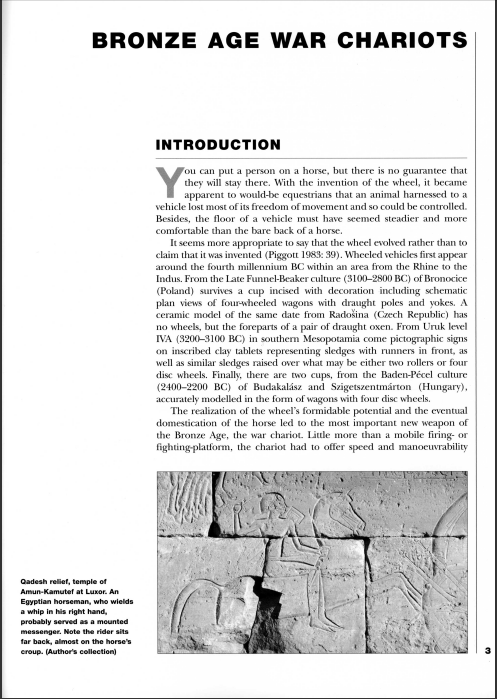
\includegraphics[width=0.5\textwidth]{./chapters/chapter22.png}}
\end{figure}

\lipsum[1-2]
\parindent0pt


\end{document}

\cxset{chapter opening=any}
\chapter{Introduction}

The development of a style template for a statistics book, following the style of Statistics for Engineers and Scientists.
The book can easily be developed by the \pkgname{phd} package.  Remember that the best way to start is to use an existing template and to modify the parameters.

\begin{docEnvironment}[doclang/environment content=key description,doc updated=2015-01-29]{docKey}{\oarg{key path}\oarg{options}\marg{name}\marg{parameters}\marg{description}}
  Documents a key with given \meta{name} and an optional \meta{key path}.
  The given \meta{options} are set with \refCom{tcbset}.
  This key takes mandatory or optional \meta{parameters} as value
  with a short \meta{description}.
  It is automatically indexed and can be referenced with
  \refCom{refKey}\marg{name}.
\begin{dispExample}
\begin{docKey}[foo]{footitle}{=\meta{text}}{no default, initially empty}
  Creates a heading line with \meta{text} as content.
\end{docKey}
\end{dispExample}
\end{docEnvironment}


\begin{docCommand}{docValue}{\marg{name}}
  Documents a value with given \meta{name}. Typically, this is a value for a key.
  This value is automatically indexed.
\begin{dispExample}
A feasible value for \refKey{/foo/footitle} is \docValue{foovalue}.
\end{dispExample}
\end{docCommand}

\begin{docCommand}[doc new=2015-01-08]{docCounter}{\marg{c@chapter}}
  Documents a counter with given \meta{name}. The counter is automatically indexed.
\begin{dispExample}
The counter \docCounter{foocounter} can be used for computation.
\end{dispExample}
\end{docCommand}


\begin{figure}[htbp]
\centering
\includegraphics[width=0.8\textwidth]{./images/statistics.jpg}
\end{figure}

I am not too very sure if the choice of color and sky blue for the sections is such a good combination, so we will try both and see which one you like.

\section{Set the Sections} 
 \arial

 The sections can easily be set using the package. We need to define some colors, the font parameters and the
 indentation into the margins. We will revisit some of the settings but for the time being the following settings will do.
 
 \begin{teX}
 \cxset{%
   section afterindent = false, 
   section color= sweet,     
   section beforeskip=15pt,
   section afterskip=15pt,
   section indent=-3cm,
   section font-family= sffamily,
   section font-size= LARGE,
   section font-weight= bfseries,
   section font-shape=,
   section align= left,
   section numbering prefix =\color{black!55}\thechapter.,
   section numbering= arabic,
   section spaceout=soul,
}
 \end{teX}



 \cxset{% 
  section numbering prefix =\thechapter.,}

\section{Examples and Solutions}

\newcounter{example}[chapter]

Obviously any book addressed to a student audience will have special sections for examples, solutions problems and answers and this was the main reason why I have introduced this particular style early in the documentation.

The examples are framed with a `T’ shaped ruler and are numbered in arabic numerals, with the chapter prefix. they are reset at every chapter.
\newlength\rulerlength
\cxset{rule color=sweet}
\color{black!85}
\makeatletter
\def\example{%
\stepcounter{example}
\settowidth{\rulerlength}{\textbf{Example 10.1}}
\addtolength{\rulerlength}{1cm}
\parindent0pt
\bgroup

\color{sweet}
\parindent-\rulerlength\relax
\leavevmode\par
\rule{\dimexpr(2\rulerlength)}{1.5pt}%
\vskip-12pt
\moveright-4pt\vbox to 0pt{\llap{\sffamily\textbf{Example \thechapter.\theexample :} \hbox to 0pt{\color{sweet}\rule{1.5pt}{\baselineskip}}}}
\egroup%
\everypar{\parindent2em}
}%

\example Suppose that an engineer encounters data from a manufacturing process in which
100 items are sampled and 10 are found to be defective. It is expected and anticipated
that occasionally there will be defective items. Obviously these 100 items
represent the sample. However, it has been determined that in the long run, the
company can only tolerate 5\% defective in the process. Now, the elements of probability
allow the engineer to determine how conclusive the sample information is
regarding the nature of the process. In this case, the population conceptually
represents all possible items from the process. Suppose we learn that if the process
is acceptable, that is, if it does produce items no more than 5\% of which are defective,
there is a probability of 0.0282 of obtaining 10 or more defective items in
a random sample of 100 items from the process. This small probability suggests
that the process does, indeed, have a long-run rate of defective items that exceeds
5\%. In other words, under the condition of an acceptable process, the sample information
obtained would rarely occur. However, it did occur! Clearly, though, it
would occur with a much higher probability if the process defective rate exceeded
5\% by a significant amount.

From this example it becomes clear that the elements of probability aid in the
translation of sample information into something conclusive or inconclusive about
the scientific system. In fact, what was learned likely is alarming information to
the engineer or manager. Statistical methods, which we will actually detail in
Chapter 10, produced a P-value of 0.0282. The result suggests that the process
very likely is not acceptable. The concept of a P-value is dealt with at length
in succeeding chapters. The example that follows provides a second illustration.

\def\solution{%
   \everypar{}
   \parindent0pt
  \leavevmode\par
  \makebox{\llap{\bfseries\textit{Solution }:}\thinspace}%
  \parindent2em
  }
 
\solution Let $X$ represent the number of good components in the sample. The probability
distribution of $X$ is\par

\lipsum[1]\par

\section{Figures}

Since the book is a mathematical textbook, it does not contain too many pictures. Captions are styled easily
with normal phd settings---as a matter of fact---the default style is ok and the looks of the page are
improved by the usage of the same sky blue color as the headings.

\begin{figure}[htbp]
\centering
\includegraphics[width=0.8\textwidth]{./images/statistics-figures.jpg}
\caption{Figures are styled after common LaTeX styles and do not need any particular treatment.}
\end{figure}

\section{Tables}

Tables are always very visual and book designers tend to spend considerable artistic effort to style them. This particular book style, just styles the captions at the primary color of the book (sky blue). Smaller tables are set
in black, including the heading.

The tables in the Appendix all have nice blue captions and some of them have also a small figure at the edge. 
Of course any TeXnician would generate these tables, nowdays using Lua. The figures can be absolute positioned
using pgf or similar methods.

\begin{figure}[htbp]
\example Reproduce the pages shown below to cater for figures.\par
\vskip\abovedisplayskip

\centering
\includegraphics[width=0.8\textwidth]{./images/statistics-tables.jpg}
\caption{Figures are styled after common LaTeX styles and do not need any particular treatment.}
\end{figure}

\lipsum[1-3]
\def\doublerule{%
\toprule
\addlinespace[0pt]
\midrule}

\begin{table}[htbp]
\example Develop a table with a double rule on top of the table head.\par
\centering 
\caption{Absorption of Moisture in Concrete Aggregates}
\label{tbl:stats}
\begin{tabular}{rrrrrr}
\doublerule
Aggregate    &1  &2 &3 &4 &5\\
\midrule
                   &551 & 595 & 639 & 417 & 563\\
\bottomrule
\end{tabular}
\end{table}

\noindent In addition, we may be interested in making individual comparisons among these
5~population means

\solution The only item we needed to define in addition to standard macros provided is the \string\doublerule.
\begin{verbatim}
\begin{table}[htbp]
\centering 
\caption{Absorption of Moisture in Concrete Aggregates}
\label{tbl:stats}
\begin{tabular}{rrrrrr}
\doublerule
Aggregate    &1  &2 &3 &4 &5\\
\midrule
                   &551 & 595 & 639 & 417 & 563\\
\bottomrule
\end{tabular}
\end{table}
\end{verbatim}



\makeatletter\@specialfalse

\cxset{
 toc image = \@empty,
 name={},
 numbering=arabic,
 number font-size= LARGE,
 number font-family= rmfamily,
 number font-weight= bfseries,
 number before=,
 number dot=,
 number after=,
 number position=leftname,
 chapter font-family= sffamily,
 chapter font-weight= normalfont,
 chapter font-size= Large,
 chapter before={\vspace*{15pt}\par},
 chapter after={\hfill\hfill\par},
 number color=black!90,
 title beforeskip={\vspace*{30pt}},
 title afterskip={\vspace*{40pt}\par},
 title before={},
 title after={},
 title font-family= sffamily,
 title font-color= black,
 title font-weight= bfseries,
 title font-size= LARGE,
 header style= plain,
 }

\cxset{headings ruled-01}

\chapter{Introduction to Style One}


\begin{summary}
This design is simple and its distinguishing characteristic is a short summary at the beginning of the chapter. This is almost like an abstract typeset in italic font without setting the margins in. We provide a \lstinline{summary} environment for convenience. Note the very simple line in the running head to the left of the page number.
\end{summary}

\medskip
\begin{figure}[ht]
\centering
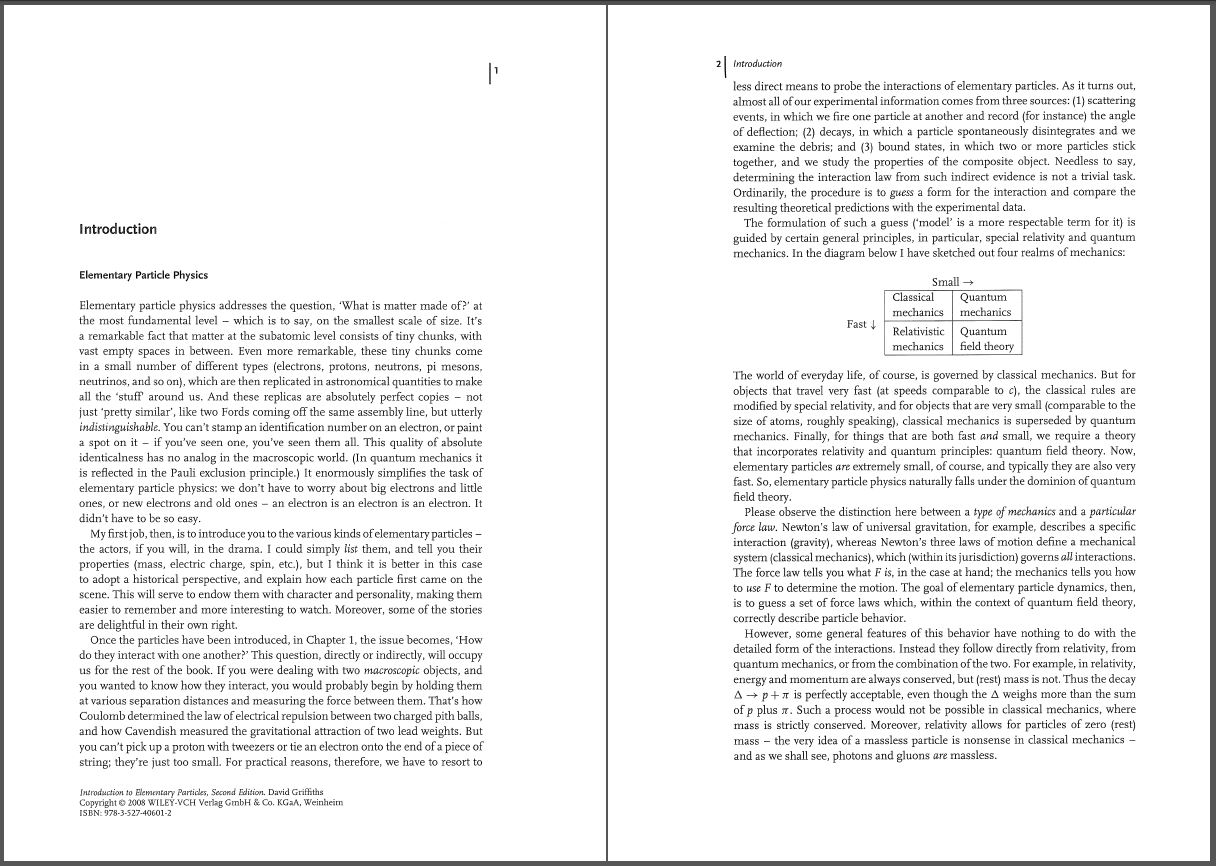
\includegraphics[width=0.5\textwidth]{./chapters/chapter01.png}
\end{figure}
\makeatother

\clearpage
\makeatletter\@debugtrue\makeatother
\cxset{
 chapter toc=true,
 name=CHAPTER,
 chapter numbering=ORDINALS,
 number font-size=Large,
 number font-family=rmfamily,
 number font-weight=bfseries,
 number before=\kern0.5em,
 number dot=,
 number after=\hfill\hfill\par,
 number position=rightname,
 chapter font-family=rmfamily,
 chapter font-weight=bold,
 chapter font-size=Large,
 chapter before={\vspace*{20pt}\par\hfill},
 chapter after=,
 chapter color=black,
 number color=black,
 %
 title margin top=10pt,
 title before=\par\nointerlineskip\hfill,
 title after=\hfill\hfill\par\nointerlineskip,
 title font-family=rmfamily,
 title font-color= black,
 title font-weight=bfseries,
 title font-size=LARGE,
 chapter title width=0.8\textwidth,
 chapter title align=centering,
 title margin-left=0pt,
 author block=false}

\debugtitle
\debugchapter
\chapter[Template 2]{Mondino, the Restorer of Anatomy}

The archive.org is an extraordinary hunting ground  for typographical surprises. On a recent excursion to find some books on Versalius I stubled on a book titled \emph{Andreas Vesalius, the reformer of anatomy} by  Ball, James Moores. It is an old book published in 1910 and has a couple of unusual features. Check the figure below and see if you can identify the challenging feature.

\begin{figure}[ht]
\centering
\includegraphics[width=0.8\textwidth]{versalius}
\caption{J.B. Moore’s \emph{Andreas Versalius, the Reformer of Anatomy} has many unusual features, including chapter numbers using ordinals. }
\end{figure}

\cxset{chapter toc=true,
          chapter opening=anywhere}
          
\chapter{The Template}          
The template is called \emph{Versalius} and is stored under style02. It can be loaded in the normal way using:
\begin{verbatim}
\usepackage[style02]{phd}
\end{verbatim}

I have not reproduced the full extend of the book’s requirements, as some details are quite cumbersome to be automated through \tex. These though can easily be incorporated in a manual way. More about this later.


\section{The Table of Contents}
Another interesting aspect of this book, which is common with many books of its period is the ToC. The ToC shows the full range of the chapter pages, i.e., it is marked as Page 1-16 rather than the common practice nowdays that indicates only the starting page of the chapter. It also has “TABLE OF CONTENTS”  as a heading and not just contents as you would expect from today’s books.

\begin{figure}[ht]
\centering
\includegraphics[width=0.8\textwidth]{versalius-01}
\caption{J.B. Moore’s \emph{Andreas Versalius, the Reformer of Anatomy} has many unusual features, including chapter numbers using ordinals. }
\end{figure}

\section{List of Illustrations}

\begin{figure}[ht]
\centering
\includegraphics[width=0.8\textwidth]{versalius-02}
\caption{J.B. Moore’s \emph{Andreas Versalius, the Reformer of Anatomy} has many unusual features, including chapter numbers using ordinals. }
\end{figure}

\section{The Frontmatter}
As a foreward there is an unumbered chapter called ``Introduction’’. The chapter heading also has a head band.
\begin{figure}[ht]
\centering
\includegraphics[width=0.8\textwidth]{versalius-03}
\caption{J.B. Moore’s \emph{Andreas Versalius, the Reformer of Anatomy} has many unusual features, including chapter numbers using ordinals. }
\label{lettrine}
\end{figure}

\bgroup
\centering
\includegraphics[width=0.7\textwidth]{versalius-headband}

\LARGE\bfseries INTRODUCTION\par
\egroup
\def\dropcapversalius{%
\vbox to 0pt{\vskip6pt\leavevmode\noindent\includegraphics[width=2.39cm]{versalius-dropcap}%
}%
}
\parindent0pt

\hangindent2.6cm \hangafter0
\dropcapversalius \textsc{he dropcap will have to be inserted}, either using the lettrine package or do be achieved via a parshape command and manual entry. You can also write your own macro command using the details we provide under the Paragraphs chapter. On this page I have manually inserted it, as I used an image from the book for the dropcap. If you were to use the template for a full book, it will be then preferable to use

the lettrine package to set the dropcaps. If you observe Figure~\ref{lettrine} carefully, you will notice the first line of theopening paragraph is in small caps. As \tex typesets the full paragraph this is almost an impossible task to achieve through normal \tex commands and in order not to overcomplicate the discussion it can be achieved manually via trial and error. 

\section{Figures}

Most of the figures are wrapped illustrations. A couple are full page figures and bear no caption numbering. One such illustration is shown on page~\pageref{fig:vesalius}. Do note that the List of Illustrations does have the illustrations listed with additional information to that shown in the captions. 

\begin{figure}[p]
\centering
\includegraphics[width=\textwidth]{vesalius}
\centering
ANDREAS VESALIUS\par
(From an old copperplate engraving)\par
\label{fig:vesalius}
\end{figure}







%\newgeometry{top=-10pt,bottom=2cm}


\cxset{style03/.style={
 toc image = \@empty,
 name={},
 numbering=arabic,
 number font-size= HUGE,
 number font-family= rmfamily,
 number font-weight= bfseries,
 number before=\par\vspace*{10pt}\hfill\hfill,
 number dot=.,
 number after=,
 number position=rightname,
 chapter font-family= sffamily,
 chapter font-weight=normalfont,
 chapter font-size= Large,
 chapter before={\hspace*{-2.5cm}\vbox\bgroup%
    \tcbset{width=\paperwidth,boxrule=0pt,right=3cm,arc=0pt}
    \tcolorbox\bgroup\vspace*{20pt}\hfill\hfill},
 chapter after={\par\vspace*{15pt}},
 chapter color=black!90,
 number color= thered,
 title beforeskip={},
 title afterskip={\vspace*{10pt}\par},
 title before={\hfill\hfill},
 title after={\vspace*{60pt}\egroup\endtcolorbox\egroup},
 title font-family=\sffamily,
 title font-color= thered,
 title font-weight=\bfseries\RaggedRight,
 title font-size=\Huge}}

\cxset{style03}

\chapter{Introduction Style Three}

This is not an exact reproduction as I am still thinking as to how to use
specials with the package. You can vary it by setting the tcolorbox settings as well as the geometry settings.
\medskip

\begin{figure}[ht]
\centering
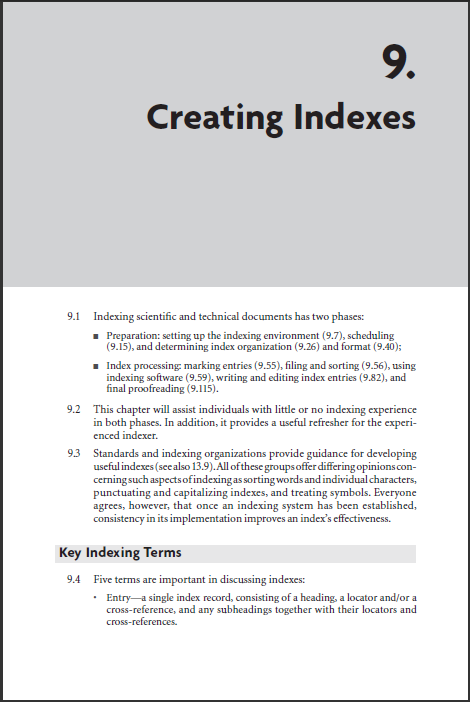
\includegraphics[width=0.39\textwidth]{./chapters/chapter03}
\end{figure}

This setting involves changing the geometry of the page as well as adding the chapter name and title in a color box. For this I have used the \lstinline{tcolorbox}. Of course you can use any other shaded environment you feel comfortable with such as mdframed. It is important to set the colorbox parameters.

\begin{lstlisting}
\newgeometry{top=-10pt}
\tcbset{width=\paperwidth,boxrule=0pt,right=3cm,arc=0pt}
\end{lstlisting}

Note that we set the width of the \lstinline{tcolorbox} to \lstinline{\paperwidth} in order for the shading to extend to the full width of the page.

\restoregeometry

\cxset{style04/.style={
 chapter name=,
 numbering=Roman,
 number font-size=Large,
 number font-family=rmfamily,
 number font-weight=bfseries,
 number before=,
 number dot=,
 number after=,
 number color=black,
 number position=rightname,
 chapter font-family= rmfamily,
 chapter font-weight=bold,
 chapter font-size=Large,
 chapter before=,
 chapter after=,
 chapter color=black!90,
 chapter border-style=none,
 chapter border-width=0pt,
 chapter display=block,
 chapter float=center,
 title beforeskip={},
% title afterskip={\vspace*{50pt}\par},
 title margin bottom=50pt,
 title margin-left=0pt,
 chapter title align=centering,
 chapter title text-align=center,
 chapter title width=\textwidth,
 title display=block,
 title border-left-width=0.2pt,
% title hooks leave emptt 
 title before=,
 title after=,
 % title families leave as default font name
 title font-family=rmfamily,
  title font-color= black,
 title font-weight=normalfont,
 title font-size=LARGE,
 % title alignment
 chapter title align=centering,
 % sectioning incomplete please add to suit
 section numbering=none,
 section align = center}}

\debugchapter
\cxset{chapter border-width=2pt,
          chapter padding=5pt,
          number border-width=2pt,
          number padding=5pt}

\cxset{style04}

\chapter{INTRODUCTION TO STYLE FOUR}

This is a very simple design applicable perhaps to translations and commentary on older texts.
\medskip
\begin{figure}[ht]
\centering
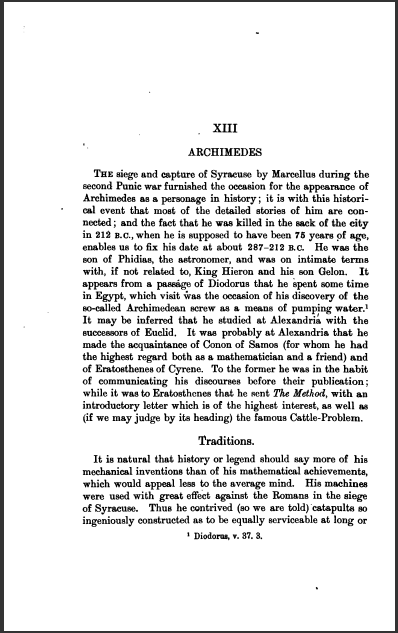
\includegraphics[width=0.6\textwidth]{./chapters/chapter04.png}
\end{figure}

\testsections



%%%%%%%%%%%%%%%%%%%%%%%%%%%%%%%%%%%%%%%%%%%
%%%%%%  STYLE 05
%%%%%%%%%%%%%%%%%%%%%%%%%%%%%%%%%%%%%%%%%%%


\cxset{style05/.style={
 name={Chapter},
 numbering=arabic,
 number font-size=\Large,
 number font-family=\rmfamily,
 number font-weight=\normalfont\itshape,
 number color=\color{black!90},
 number before=,
 number dot=,
 number after=,
 number position=rightname,
 chapter font-family=\rmfamily,
 chapter font-weight=\normalfont\itshape,
 chapter font-size=\Large,
 chapter before={\hrule width \columnwidth \kern2.6pt \par\hfill},
 chapter after={\hfill\hfill\par},
 chapter color={black!90},
 chapter spaceout=none,
 title beforeskip={\vspace*{10pt}},
 title afterskip={\vspace*{50pt}\par},
 title before={\hfill},
 title after={\hfill\hfill \vskip2.6pt\hrule width \columnwidth \kern2.6pt },
 title font-family=\rmfamily,
 title font-color=\color{black!90},
 title font-weight=\bfseries,
 title font-size=\huge,
 header style= headings}}

\cxset{style05}
\chapter{Introduction to Style Five}\index{ch:style5}

\tcbset{width=\textwidth}
I think this style can be improved with a bit of color. You can experiment with it quite easily. The spacing on top of this style can also be adjusted to suit your typographical taste.
\medskip
\begin{figure}[ht]
\centering
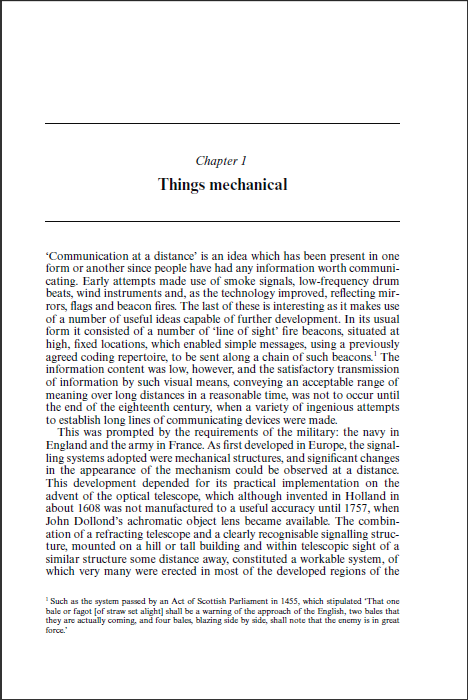
\includegraphics[width=0.6\textwidth]{./chapters/chapter05}
\end{figure}

%\section{General notes on rules}

LaTeX's default rules would normally give problems. Best is to use TeX's primitives to built them.

%\index{rules!example color}
%\begin{texexample}{}{}
%\makeatletter
%\hrule width 5cm \kern2.6\p@
%AAAAAAAAAAAAAAAAAAAAA
%\vskip2.6pt\hrule width 5cm
%\medskip
%
%Problem with LaTeX rules.
%
%\rule{5cm}{0.4pt}\par
%AAAAAAAAAAAAAAAAAAAAA\par%
%\rule[6.5pt]{5cm}{0.4pt}
%
%\def\rule{\@ifnextchar[\@rule{\@rule[\z@]}}
%\def\@rule[#1]#2#3{%
% \leavevmode
% \hbox{%
% \setlength\@tempdima{#1}%
% \setlength\@tempdimb{#2}%
% \setlength\@tempdimc{#3}%
% \advance\@tempdimc\@tempdima%
% \vrule\@width\@tempdimb\@height\@tempdimc\@depth-\@tempdima}}
%
%\def\thickrule{\leavevmode \leaders \hrule height 3pt \hfill \kern \z@}
%
%{\color{teal}\hrule width 10.5cm height3pt \kern2.6\p@
%    {{\color{black!80}\HUGE CHAPTER TITLE}}\vskip3pt
%\hrule width 10.5cm height3pt}
%\makeatother
%\end{texexample}

%<<<<<<< HEAD
%%%%%%%%%%%%%%%%%%%%%%%%%%%%%%%%%%%%%%%%%%%
%%%%%%  STYLE 06
%%%%%%%%%%%%%%%%%%%%%%%%%%%%%%%%%%%%%%%%%%%

\cxset{style06/.style={
 name={Chapter},
 numbering=arabic,
 number font-size=\Huge,
 number font-family=\calligra,
 number font-weight=\calligra,
 number color=\color{black!90},
 number before=\kern-2.5pt,
 number dot=,
 number after=,
 number position=rightname,
 chapter font-family=\rmfamily,
 chapter font-weight=\calligra,
 chapter font-size=\LARGE\calligra,
 chapter before={\vspace*{20pt}\par\hfill},
 chapter after={\hfill\hfill\par},
 chapter color={black!90},
 title beforeskip={\vspace*{50pt}},
 title afterskip={\vspace{3.5pt}\par},
 title before={\hfill},
 title after={\hfill\hfill},
 title font-family=\rmfamily,
 title font-color=\color{black!90},
 title font-weight=\normalfont,
 title font-size=\LARGE,
 title spaceout=soul,
}}

\cxset{style06}

\chapter{INTRODUCTION TO STYLE SIX}
\renewcommand{\DefaultLhang}{0.1}
\renewcommand{\LettrineFontHook}{\calligra}
\setlength{\DefaultFindent}{9.5pt}
\setlength{\DefaultNindent}{0pt}

\lettrine{\textcolor{orange}{T}}{}he calligraphic font for this design make it stand out, although you may need to experiment to get the right font (I have used calligra). I am sure the specification can be optimized a bit, however so far it works. I also opted to space out the title. I had to experiment a bit to get the Lettrine settings.
\medskip
\begin{figure}[ht]
\centering
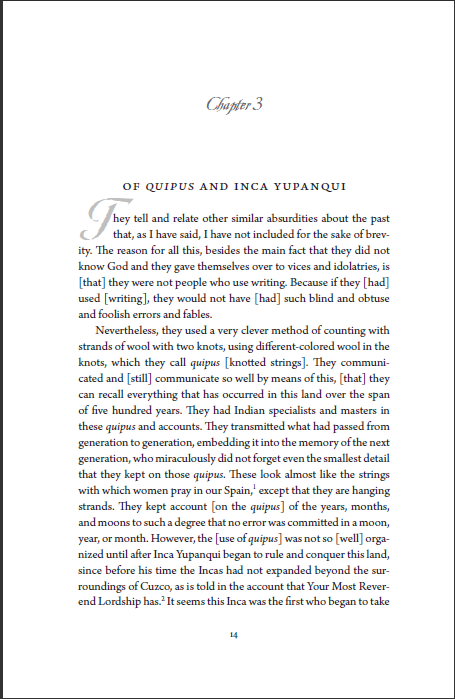
\includegraphics[width=0.6\textwidth]{./chapters/chapter06}
\end{figure}

The number has been kerned using:

\begin{lstlisting}
 number before=\kern-4.5pt,
\end{lstlisting}

This template has a lot of potential and I will come back to it and add more key hooks for lettrine settings per letter and font management. They can also come alive with a gold color.

=======
%%%%%%%%%%%%%%%%%%%%%%%%%%%%%%%%%%%%%%%%%%%
%%%%%%  STYLE 06
%%%%%%%%%%%%%%%%%%%%%%%%%%%%%%%%%%%%%%%%%%%

\cxset{style06/.style={
 name={Chapter},
 numbering=arabic,
 number font-size=\Huge,
 number font-family=\calligra,
 number font-weight=\calligra,
 number color=\color{black!90},
 number before=\kern-2.5pt,
 number dot=,
 number after=,
 number position=rightname,
 chapter font-family=\rmfamily,
 chapter font-weight=\calligra,
 chapter font-size=\LARGE\calligra,
 chapter before={\vspace*{20pt}\par\hfill},
 chapter after={\hfill\hfill\par},
 chapter color={black!90},
 title beforeskip={\vspace*{50pt}},
 title afterskip={\vspace{3.5pt}\par},
 title before={\hfill},
 title after={\hfill\hfill},
 title font-family=\rmfamily,
 title font-color=\color{black!90},
 title font-weight=\normalfont,
 title font-size=\LARGE,
 title spaceout=soul,
}}

\cxset{style06}

\chapter{INTRODUCTION TO STYLE SIX}
\renewcommand{\DefaultLhang}{0.1}
\renewcommand{\LettrineFontHook}{\calligra}
\setlength{\DefaultFindent}{9.5pt}
\setlength{\DefaultNindent}{0pt}

\lettrine{\textcolor{orange}{T}}{}he calligraphic font for this design make it stand out, although you may need to experiment to get the right font (I have used calligra). I am sure the specification can be optimized a bit, however so far it works. I also opted to space out the title. I had to experiment a bit to get the Lettrine settings.
\medskip
\begin{figure}[ht]
\centering
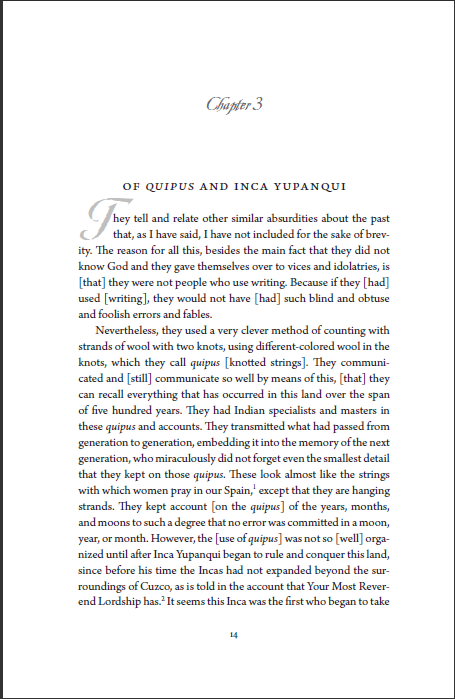
\includegraphics[width=0.6\textwidth]{./chapters/chapter06}
\end{figure}

The number has been kerned using:

\begin{lstlisting}
 number before=\kern-4.5pt,
\end{lstlisting}

This template has a lot of potential and I will come back to it and add more key hooks for lettrine settings per letter and font management. They can also come alive with a gold color.

>>>>>>> merged


\newgeometry{top=2cm,bottom=2cm,left=3cm,right=3cm}

\setdefaults

\cxset{style07/.style={
 name={},
 chapter toc=true,
 numbering=arabic,
 number font-size=HUGE,
 number font-family=sffamily,
 number font-weight=bfseries,
 number before=,
 number dot=,
 number color= gray,
 number after=\par,
 number position=leftname,
 chapter font-family=\sffamily,
 chapter font-weight=\normalfont,
 chapter font-size=\Large,
 chapter before={\hfill\hfill\hfill\par},
 chapter after={\vspace*{20pt}},
 chapter color= black!90,
 title beforeskip={\vspace*{30pt}},
 title afterskip={\vspace*{50pt}\par},
 title before={},
 title after={\par\rule[17pt]{\textwidth}{0.4pt}},
 title font-family=\sffamily,
 title font-weight=\bfseries,
 title font-size=\LARGE,
 title font-shape=normal,
 title font-color=black!90,
 title spaceout=none,
}}

\cxset{style07}
\chapter{Introduction to Style Seven}

\parindent0pt
\lipsum[1]
\medskip
\begin{figure}[ht]
\centering
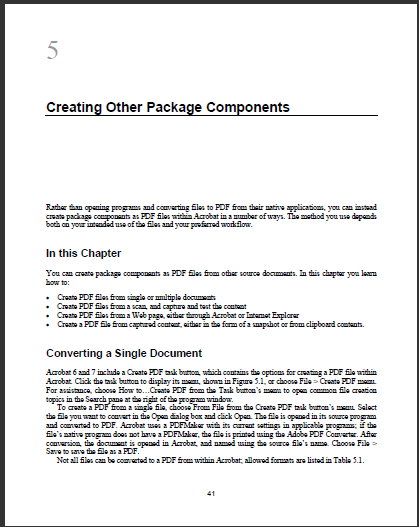
\includegraphics[width=0.6\textwidth]{./chapters/chapter07.png}
\end{figure}
\lipsum[1]

\clearpage

\setdefaults

\makeatletter
\cxset{style08/.style={
 name={},
 chapter toc=true,
 numbering=arabic,
 number font-size=\LARGE,
 number font-family=\sffamily,
 number font-weight=\bfseries,
 number color= black!90,
 number before=,
 number dot=,
 number after=,
 number position=rightname,
 chapter font-family=sffamily,
 chapter font-weight=normalfont,
 chapter spaceout=none,
 chapter font-size=Large,
 chapter before=,
 chapter after=,
 chapter color={black!90},
 chapter float=right,
 chapter display=block,
 chapter border-style=none,
 chapter border-width=0pt,
 number spaceout=none,
 number display=block,
 number float=right,
 chapter title width=0.6\textwidth,
 title beforeskip=,
 title afterskip=,
 title before=,
 title after={},
 title font-family=sffamily,
 title font-color=black!90,
 title font-weight=bfseries,
 title font-size=LARGE,
 title display=block,
 chapter title align=right,
 author block=true,
 author block format=\par\addvspace{12pt}\normalfont\large\raggedleft,
 author names=Yiannis Lazarides\par Larnaka,
 section number after=,
 section numbering = arabic,
 section numbering prefix=,
 section numbering custom = \@arabic\c@section.\space,
 section color=black,
 section numbering suffix=,
 header style=empty}}
 
 % humanized name of the style, with a non human connotation!
 %
 \cxset{humanoid/.style={style08}}
\makeatother

\cxset{section color=sweet,
          section font-shape=sffamily}


\cxset{style08}
% set the counter needs this to be modified to be based on a key value interface
\cxset{figure numbering/.is choice,
          figure numbering/within/.code=\counterwithin{figure}{chapter},
          figure numbering/without/.code=\counterwithout{figure}{chapter}}
\cxset{table numbering/.is choice,
          table numbering/within/.code=\counterwithin{table}{chapter},
          table numbering/without/.code=\counterwithout{table}{chapter}}          
%\counterwithout{figure}{chapter}

\cxset{figure numbering=without,
          table numbering=without}

\captionsetup[figure]{format = plain,    
                                 width=.67\textwidth,
                                 justification=justified,
                                 singlelinecheck=false,
                                 name=Fig.,
                                 labelsep=period,
                                 oneside,
                                 margin=0pt,
                                 font={normalsize,up}
                                 }
\captionsetup[table]{format = plain,    
                                 justification=justified,
                                 singlelinecheck=false,
                                 labelsep=period,
                                 oneside,
                                 margin=0pt,
                                 labelfont={up,it,normalfont}
                                 }
\chapter[Style 08]{Introduction to Book Style Eight Some Old Fashioned Stops}
\label{st:eight}
\section{Introduction}

This style is suited for Academic publishing, where editors are still a bit old fashioned and require that stops are placed after section numbers, but they do not require that the first line of paragraphs are indented. Any way the good folks that published this book, knew their Affective Computing well and amongst belly dancing  robots and smiling and angry faces, typography can take second place.\footnote{Jimmy Or (\textit{editor}). Affective Computing
Focus on Emotion Expression,
Synthesis and Recognition, May 2008.
}

\example 
\medskip
\begin{figure}[ht]
\centering
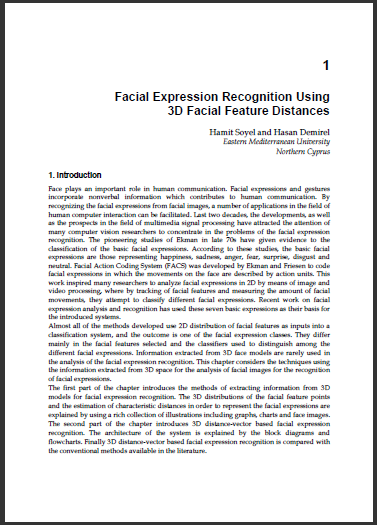
\includegraphics[width=0.5\textwidth]{./chapters/chapter08.png}
\caption{The opening page of a chapter in \textit{Affecting Computing}.}
\end{figure}

\solution To add the dot after the number can be done either using the key
\begin{verbatim}
\cxset{section numbering custom = \@arabic\c@section.,}
\end{verbatim}
or by using the pre-built key
\begin{verbatim}
\cxset{section number after=.}
\end{verbatim}

The author block including the institution are added as part of the chapter head styling command.

\example The subject of having articles together in a publication such as Proceedings and Journals is a recurring theme in many Academic fields. One of course if it is possible would have liked to use a standard Journal class and automatically produce this type of publication. There are a number of such classes at \href{http://ctan.org/tex-archive/macros/latex/required/amslatex/amscls/doc/instr-l.pdf}{ctan}

\solution If you are the editor with the task of assembling all these different articles consider using the \pkgname{confproc}. The package by Vincent Verfaille assembles the proceedings from the pdfs, using the 
\pkgname{pdfpages}, which is another great way to achieve this. A simpler way is to develop a specific style for
your Conference and let the participants use it while writing their papers. Only caveat they need to import the
body of the paper with \string\input\meta{article name}. As the \pkgname{phd} comes pre-packaged with
numerous packages the chance of someone using a package that the editor or the system needs to use it
is minimized. Indexing, bibliographies and the like might need to be taken care of and this is discussed in the relevant chapters. There are many options and peculiarities that might not be covered by the phd package so my suggestion is to try it on a few older papers first.

\example  Style-08 has to set the caption style to include for a period after the label number as shown in the Fig.~\ref{fig:eight02}. This can be achieved through key settings or a package.
\begin{figure}[ht]
\centering
\includegraphics[width=\textwidth]{./images/affective-computing.jpg}
\caption{Figures are centered, with the caption flush left and the \textit{Figure} label abbreviated to Fig. (with a stop). The section number also has the dot and follows the style of the sections.}
\label{fig:eight02}
\end{figure}

The figures numbers are reset at every chapter. Normally authors use the \pkgname{chngctr} to achieve such changes, which involves two modifications. Redefining whether or not the figure counter will be reset whenever the chapter/section counter is incremented; Redefining the "appearance" of the figure counter (\string\thefigure), i.e., removing (or adding) the chapter/section prefix.


The standard solution – which deals with modifications 1 and 2 mentioned above – is to use the \string\counterwithout and \string\counterwithin macros of the \texttt{chngcntr package}.\footnote{\protect\url{http://tex.stackexchange.com/questions/28333/continuous-v-per-chapter-section-numbering-of-figures-tables-and-other-docume}} 


\section{Tables}

The Tables follow the style for figures as far as captioning. They are all framed and although there is a genuine distain in the \latexe community for this type of style, I must admit that they are blending well with the style of this book. Another typographical tradition that has been broken in this book is that the table captions are placed below the table and not above.

\example
\begin{figure}[ht]
\centering
\includegraphics[width=\textwidth]{./images/affective-computing-tables.jpg}
\caption{Figures are centered, with the caption flush left and the \textit{Figure} label abbreviated to Fig. (with a stop). The section number also has the dot and follows the style of the sections.}
\label{fig:eight02}
\end{figure}


\begin{verbatim}
\cxset{table numbering=without}
\end{verbatim}

\setlength\extrarowheight{5pt}

\bgroup
\begin{table}[h]
\begin{tabularx}{\textwidth}{|c|c|c|X|}
\hline
Affective Movement & Mean & Standard Deviation &\RaggedRight Standard Error of the Mean\\
\hline
confident & (0.150,0.100,0.150) & (0.362,0.304,0.362)&(0.57,0.48,0.57)\\
\hline
\end{tabularx}
\caption{The table style of the book, with the caption below. You may need to increase the cell lengths.}
\end{table}
\egroup

The cell heights of the table have been increaded by 5pt, using,
\begin{verbatim}
\setlength\extrarowheight{5pt}
\end{verbatim}

\section{Front Matter}

The Front Matter includes a Title Page, Table of Contents and a Preface. Nothing special or exciting here with the exception of the Table of Contents which is a bit on the difficult side. 

\begin{figure}[ht]
\centering
\includegraphics[width=\textwidth]{./images/affecting-computing-contents.jpg}
\caption{Figures are centered, with the caption flush left and the \textit{Figure} label abbreviated to Fig. (with a stop). The section number also has the dot and follows the style of the sections.}
\label{fig:eight02}
\end{figure}

\section{Back Matter}



For the handling of the References there are numerous options and these are discussed under the Bibliography and References chapter.\footnote{\protect\url{http://tex.stackexchange.com/questions/87991/putting-bibliographies-at-the-end-of-each-chapter}} The referencing styles within paragraphs of text are author year in square brackets. I leave this to you.

\begin{figure}[ht]
\centering
\includegraphics[width=\textwidth]{./images/affective-computing-references.jpg}
\caption{Figures are centered, with the caption flush left and the \textit{Figure} label abbreviated to Fig. (with a stop). The section number also has the dot and follows the style of the sections.}
\label{fig:eight02}
\end{figure}

\parindent1em

There are no book divisions, such as an Index at the back of the book, but each chapter has its own references section, styled as a section. The occassional single Appendix appears at the end of a chapter, styled after sections and with no numbering marks.

\section{Concluding Remarks}

This template has a unique character and in my opinion deserves a bit better. Styling for algorithms, computer code additional floating sections and an index is not provided in the template and is left open for the user. It works well with the book class and with the KOMA classes. I have also given it an alias \emph{humanoid}\footnote{From one of the chapters in the book discussing the development of humanoids that can express emotions. The scientific field of human emotions and its applications both on the web as well as robotics is a vast topic. I did waste a lot of time reading the book rather than developing the style. } A minimal to use the template is shown below:

\section{Front Matter}
\begin{figure}[ht]
\centering
\includegraphics[width=\textwidth]{./images/facial-expression-1.jpg}
\caption{Figures are centered, with the caption flush left and the \textit{Figure} label abbreviated to Fig. (with a stop). The section number also has the dot and follows the style of the sections.}
\label{fig:eight02}
\end{figure}


\begin{verbatim}
\documentclass{book}
\usepackage{phd}
\cxset{humanoid}
\begin{document}
... contents
\end{document}
\end{verbatim}

If you do restyle it, please let me know with samples of the work.

\begin{key}{/phd/section align=center}{initial none}

\end{key}




\cxset{author block=false}
\clearpage
\cxset{
 chapter name=none,
 numbering=arabic,
 number font-size=LARGE,
 number font-family=sffamily,
 number font-weight=mdseries,
 number before=,
 number dot=,
 number display=block,
 number float=left,
 number after={\vrule width2cm height0.4pt depth0pt\relax},
 number position=rightname,
 chapter font-family=sffamily,
 chapter font-weight=normalfont,
 chapter font-size=Large,
 chapter before={\vspace*{10pt}\par},
 chapter after={},
 chapter color={black!90},
 number color= black!90,
 title beforeskip=,
%title afterskip={\vspace*{50pt}\par},
 title margin bottom=40pt,
 title before=,
 title after=,
 title font-family=sffamily,
 title font-color= black,
 title font-weight=normalfont,
 title font-size=LARGE,
 chapter title align=none,
chapter title text-align=left,
chapter title width=\textwidth,
 title margin top=0pt,
 section numbering=none,
 section font-weight=normalfont,
 section indent=0pt,
 section align=centering,
 }
 \renewsection
\chapter{Preparing for Trial}

Template number nine, is from a book about a the Rivonia Trial. The template is easy to set up and is has a simple but effective design, which I think is very appropriate for a journalistic type of book. 
\medskip
\begin{figure}[ht]
\centering
\hspace*{-.1\textwidth}{\color{thegray}\fbox{\includegraphics[width=1.2\textwidth]{mandela-01}}}
\end{figure}

When South Africa's apartheid government charged Nelson Mandela with planning its overthrow in 1963, most observers feared that he would be sentenced to death. But the support he and his fellow activists in the African National Congress received during his trial not only saved his life, but also enabled him to save his country. In Saving Nelson Mandela, South African law expert Kenneth S. Broun recreates the trial--called the ``Rivonia" Trial after the Johannesburg suburb where police seized Mandela. Based upon interviews with many of the case's primary figures and portions of the trial transcript, Broun situates readers inside the courtroom at the imposing Palace of Justice in Pretoria. Here, the trial unfolds through a dramatic narrative that captures the courage of the accused and their defense team, as well as the personal prejudices that colored the entire trial. The Rivonia trial had no jury and only a superficial aura of due process, combined with heavy security that symbolized the apartheid government's system of repression. 

Broun shows how outstanding advocacy, combined with widespread public support, in fact backfired on apartheid leaders, who sealed their own fate. Despite his 27-year incarceration, Mandela's ultimate release helped move his country from the racial tyranny of apartheid toward democracy. As documented in this inspirational book, the Rivonia trial was a critical milestone that helped chart the end of Apartheid and the future of a new South Africa.

``Kenneth Broun does justice indeed to one of the most celebrated political trials of the 20th century...the result is not only a gripping story but a work of profound scholarship, sensitivity, and empathy." --Mark Gevisser, author of A Legacy of Liberation 

``Part history, part sociology, part engrossing legal drama, this important book recounts a seminal moment in South Africa's history." --Penelope Andrews, City University of New York School of Law

Many things are going wrong in South Africa, but it would have been worse if it was not for Mandela.  

To use the template simply load the \pkgname{phd} package and |style09| or |rivonia|. Adjust spacing fonts and geometry to your liking:

\begin{verbatim}
\documentclass{book}
\usepackage{phd}
\phdusetemplate{style09}
\cxset{chapter opening=anywhere}
\begin{document}
\chapter{Arrests and Escapes}
\end{document}
\end{verbatim}

\cxset{chapter opening=anywhere}

\chapter{Arrests and Escapes}

\lorem

\section{Adjusting the Rule}

You might want to fiddle with the rule settings, as well as the section settings. I prefer the sections centered and not numbered.

\thispagestyle{headings}









<<<<<<< HEAD
%%%%%%%%%%%%%%%%%%%%%%%%%%%%%%%%%%%%%%%%%%%
%%%%%%  STYLE 10
%%%%%%%%%%%%%%%%%%%%%%%%%%%%%%%%%%%%%%%%%%%

\cxset{
 name=CHAPTER,
 numbering=WORDS,
 number font-size=\huge,
 number font-family=\sffamily,
 number font-weight=\bfseries,
 number before=,
 number dot=,
 number after=\hspace{1em},
 number position=rightname,
 chapter font-family=\sffamily,
 chapter font-weight=\bfseries,
 chapter font-size=\huge,
 chapter before={\vspace*{0.4\textheight}\hfill},
 chapter after={\hfill\hfill\vskip0pt\thinrule\par},
 chapter color={black!90},
 number color=\color{black!90},
 title beforeskip={\vspace*{30pt}},
 title afterskip={\vspace*{30pt}\par},
 title before={\hfill},
 title after={\hfill\hfill},
 title font-family=\sffamily,
 title font-color=\color{black!90},
 title font-weight=\bfseries,
 title font-size=\huge,
 section font-size=\LARGE,
 section font-weight=\normalfont,
 section font-family=\sffamily,
 section align=,
 section numbering=none,
 section indent=-1em,
 section align=\centering,
 section beforeskip=20pt,
 section afterskip=10pt,
 section spaceout=soul,
 section font-shape=,
}

 %set the sectioning commands


\renewsection

\chapter{INTRODUCTION TO STYLE TEN}

\section{Basic Description:}
This chapter style has the unique characteristic that the chapter number is spelled out, rather than being in arabic numerals. The setting for this is the option \lstinline{numeric=WORDS}. Use either a capital for uppercase or \lstinline{numeric=words} for lowercase number labels.

\medskip
\begin{figure}[ht]
\centering
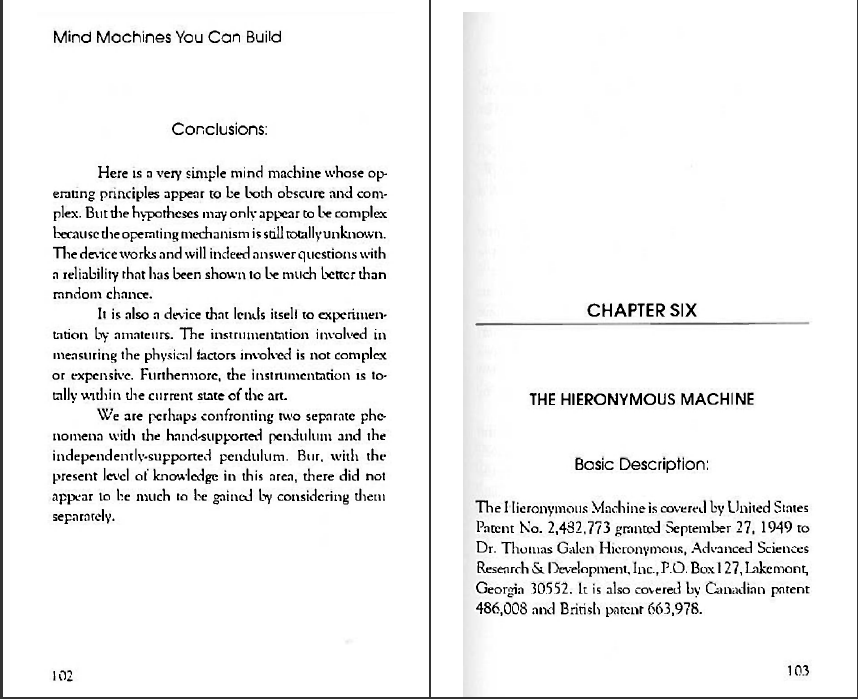
\includegraphics[width=0.6\textwidth]{./chapters/chapter10}
\end{figure}

\lipsum[1]
=======
%%%%%%%%%%%%%%%%%%%%%%%%%%%%%%%%%%%%%%%%%%%
%%%%%%  STYLE 10
%%%%%%%%%%%%%%%%%%%%%%%%%%%%%%%%%%%%%%%%%%%

\cxset{
 name=CHAPTER,
 numbering=WORDS,
 number font-size=\huge,
 number font-family=\sffamily,
 number font-weight=\bfseries,
 number before=,
 number dot=,
 number after=\hspace{1em},
 number position=rightname,
 chapter font-family=\sffamily,
 chapter font-weight=\bfseries,
 chapter font-size=\huge,
 chapter before={\vspace*{0.4\textheight}\hfill},
 chapter after={\hfill\hfill\vskip0pt\thinrule\par},
 chapter color={black!90},
 number color=\color{black!90},
 title beforeskip={\vspace*{30pt}},
 title afterskip={\vspace*{30pt}\par},
 title before={\hfill},
 title after={\hfill\hfill},
 title font-family=\sffamily,
 title font-color=\color{black!90},
 title font-weight=\bfseries,
 title font-size=\huge,
 section font-size=\LARGE,
 section font-weight=\normalfont,
 section font-family=\sffamily,
 section align=,
 section numbering=none,
 section indent=-1em,
 section align=\centering,
 section beforeskip=20pt,
 section afterskip=10pt,
 section spaceout=soul,
 section font-shape=,
}

 %set the sectioning commands


\renewsection

\chapter{INTRODUCTION TO STYLE TEN}

\section{Basic Description:}
This chapter style has the unique characteristic that the chapter number is spelled out, rather than being in arabic numerals. The setting for this is the option \lstinline{numeric=WORDS}. Use either a capital for uppercase or \lstinline{numeric=words} for lowercase number labels.

\medskip
\begin{figure}[ht]
\centering
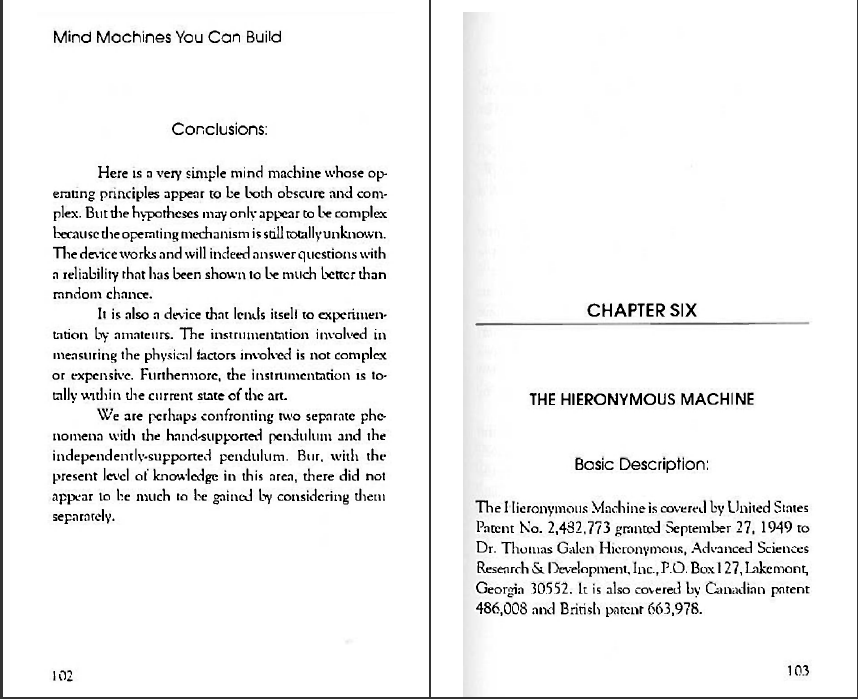
\includegraphics[width=0.6\textwidth]{./chapters/chapter10}
\end{figure}

\lipsum[1]
>>>>>>> merged

\cxset{style11/.style={
 chapter opening=any,
 name=Chapter,
 numbering=arabic,
 number font-size=LARGE,
 number font-family=rmfamily,
 number font-weight=bfseries,
 number before=,
 number dot=,
 number after=,
 number before=\kern0.5em,
 number display=inline,
 number float=center,
 chapter display=block,
 chapter float=center,
 chapter font-family=rmfamily,
 chapter font-weight=bfseries,
 chapter font-size=LARGE,
 chapter before=,
 chapter after=,
 chapter color=black!90,
 chapter spaceout=none,
 chapter border-width=0pt,
 chapter border-style=none,
 number color=black!90,
 title beforeskip=,
 title afterskip=,
 title before=,
 title after=,
 title font-family=rmfamily,
 title font-color=black!90,
 title font-weight=bfseries,
 title font-size=LARGE,
 chapter title width=\textwidth,
 chapter title align=centering,
 section afterindent=true,
 section align=left,
 section numbering=arabic,
 section numbering prefix=\thechapter.,
 section numbering suffix=\space,
 section indent=0pt,
 section font-family=rmfamily,
 }}
\renewsection\renewsubsection

\cxset{style11}
\chapter{\textit{Elements} II and Babylonian Metric Algebra, Introduction to Style Eleven}

The origins of Greek Mathematics, according to the Greeks is Egypt and according to J\"oran Friberg is Babylonia. This template is based on Friberg's book \emph{Amazing Traces of a Babylonian Origin in Greek Mathematics}. The book was published by World Scientific in 2007. The book size is $5.97\times8.88$ inches and uses a variety of fonts, with the main document font in Times. 

\medskip
\begin{figure}[ht]
\centering
\fbox{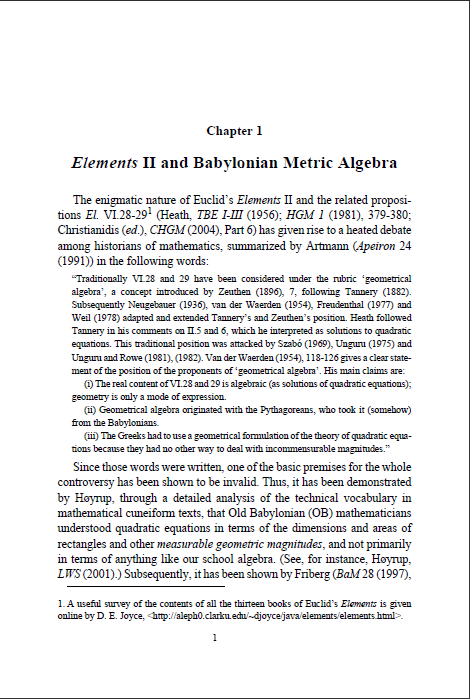
\includegraphics[width=0.65\textwidth]{./chapters/chapter11.png}}
\end{figure}
\lipsum[1]

\section{Indentation}

The book follows swedish traditional typography with the paragraphs following subheadings indented. This is achieved in the template using:

\begin{verbatim}
\cxset{section afterindent=true}
\end{verbatim}

\section{Images}
\indent Images and their captions follow a \latexe style and I am sure the book must have been styled using a \latexe xml clone as the book's pdf was produced with iText\footnote{\url{http://itextpdf.com/}}.

\begin{figure}[ht]
\centering
\includegraphics[width=0.8\textwidth]{greekmaths}
\caption{Extract from the \textit{Amazing Traces of Babylonian Influence in Greek Mathematics.} Note the styling of the caption.}
\end{figure}

\testsections

% reset for following chapters
\cxset{section afterindent=false}


\parindent0pt
\makeatletter
\cxset{style12/.style={%
 chapter name=,
 chapter toc=true,
 chapter numbering=arabic,
 number font-size=HUGE,
 number font-family=rmfamily,
 number font-weight=bfseries,
 number before=,
 number dot=,
 number color= gray,
 number after=,
 number position=rightname,
 number float=left,
 number display=block,
 chapter font-family=sffamily,
 chapter font-weight=normalfont,
 chapter font-size=huge,
 chapter before=,
 chapter after=,
 chapter color={black!90},
 title beforeskip={\vspace*{0pt}},
 title afterskip={\vspace*{50pt}\par},
 title before=,
 title after={\par\vspace{20pt}\rule{\textwidth}{4pt}},
 title font-family=sffamily,
 title font-color=black!90,
 title font-weight=bfseries,
 title font-size=Huge,
 title font-shape=normal,
 title spaceout=none,
 chapter title width=.8\textwidth,
 chapter title align=left,
 chapter title text-align =left,
}}
\makeatother

\cxset{style12}
\chapter{Why Have They Become Mainstream so Quickly? }
\label{ch:style12}
This is a variation of Style 7, with only the lettering and the rule are thicker. In my opinion it looks better with a bit of color, so I have used a purple color with a gray.

\medskip
\begin{figure}[ht]
\centering
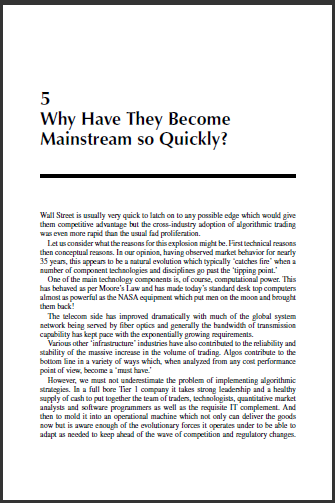
\includegraphics[width=0.35\textwidth]{./chapters/chapter12.png}
\caption{Style 12 sample from the book.}
\end{figure}
\lipsum[1]


%%%%%%%%%%%%%%%%%%%%%%%%%%%%%%%%%%%%%%%%%%%
%%%%%%  STYLE 15
%%%%%%%%%%%%%%%%%%%%%%%%%%%%%%%%%%%%%%%%%%%
\newgeometry{left=2cm,right=7cm, marginparsep=15pt, marginparwidth=4.2cm,top=2cm}
\cxset{
 name={},
 numbering=none,
 number font-size=\LARGE,
 number font-family=\rmfamily,
 number font-weight=\bfseries,
 number before=,
 number dot=,
 number after=,
 number position=rightname,
 chapter font-family=\sffamily,
 chapter font-weight=\normalfont,
 chapter font-size=\Large,
 chapter before={},
 chapter after={},
 chapter color={black!90},
 number color=\color{purple},
 title beforeskip={},
 title afterskip={\vspace*{50pt}\par},
 title before={},
 title after={},
 title font-family=\rmfamily,
 title font-color=\color{black!80},
 title font-weight=\normalfont,
 title font-size=\Huge,
 title font-shape=\itshape,
 chapter opening=any,
 watermark text=SAMPLE PAGE,
 header style=samplepage}


\chapter{Introduction to Style Fifteen}

\parindent1em
\def\thefigure{\arabic{chapter}.\arabic{figure}}
\lorem\par

\marginpar{%
 {\centering
 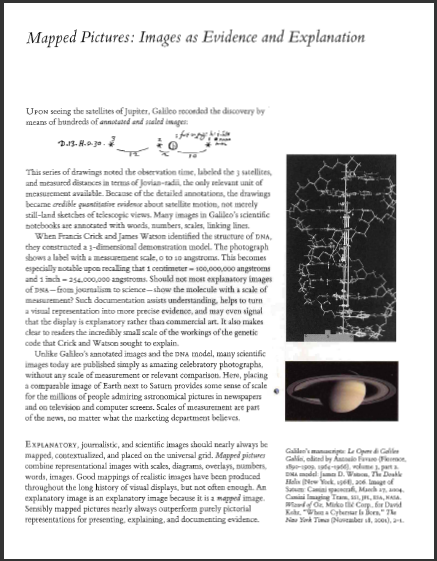
\includegraphics[width=4.2cm]{./chapters/chapter15}\vskip5pt\par}
 {\footnotesize\lorem}
}
\marginpar{%
{\centering
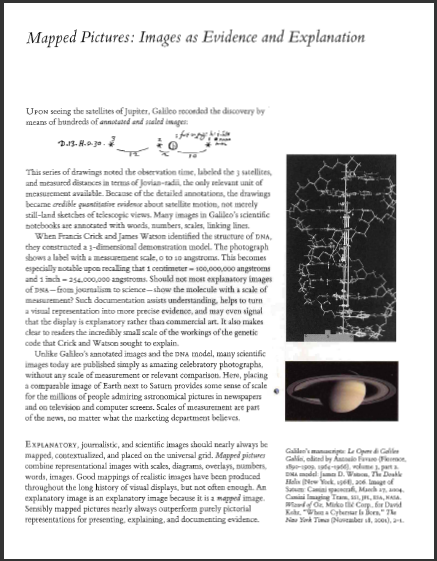
\includegraphics[width=4.2cm]{./chapters/chapter15}\par}
 { \captionof{figure}{\footnotesize\lorem}}
}
This is another marginpar of the same size.

\lorem

\lipsum
\marginpar{%
{\centering
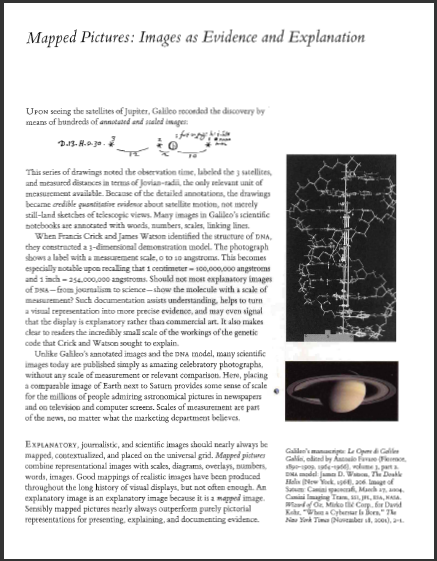
\includegraphics[width=4.2cm]{./chapters/chapter15}\par}
 { \captionof{figure}{\footnotesize\lorem}}
}
%%%% END STYLE %%%%%%%%%%%%%%%%%%%%%%%%%%%%%%%%%


\newgeometry{left=7.5cm,right=2cm, marginparsep=15pt, marginparwidth=4.2cm,top=2cm}
%%%%%%%%%%%%%%%%%%%%%%%%%%%%%%%%%%%%%%%%%%%
%%%%%%  STYLE 16
%%%%%%%%%%%%%%%%%%%%%%%%%%%%%%%%%%%%%%%%%%%


\cxset{style16/.style={
 chapter opening=anywhere,
 name={},
 numbering=arabic,
 number color=\color{thegray},
 number font-size=\HHUGE,
 number font-family=\rmfamily,
 number font-weight=\bfseries,
 number before=\leftskip-4cm\vbox to 0cm\bgroup\vspace*{5cm},
 number after=\egroup\vskip0pt\par,
 number dot=,
 number position=leftname,
 chapter font-family=\sffamily,
 chapter font-weight=\normalfont,
 chapter font-size=\Large,
 chapter before={},
 chapter after={\begin{picture}(0,0)
                          \put(-50pt,\dimexpr-\textheight+\footskip+20pt\relax){\parbox{\marginparwidth}{\textbf{Napoleon}\par\lorem}}%
                        \end{picture}},
 chapter color={black!90},
 title beforeskip={\par\hspace*{4cm}\thinrule\vskip0pt\hspace*{4cm}\vbox\bgroup},
 title afterskip={\vspace*{50pt}\par\egroup},
 title before={},
 title after=,
 title font-color=\color{black!80},
 title font-weight=\normalfont,
 title font-family=\rmfamily,
 title font-shape=\upshape,
 title font-size=\HUGE,
 header style=empty,
 subsection numbering=none,
 subsection color=teal,
 subsection align=\color{teal},
 header style=empty,
 }}

\renewsubsection

%%%% VERSO NAPOLEON %%%%%%%%%%%
% We define a macro to set the page dimensions to full.
% We also require the parindent to be set to 0pt and to restore it afterwards.
\def\fullpageimage{%
       \vspace*{-2.5cm}
        \parindent0pt
       \hspace*{-2cm}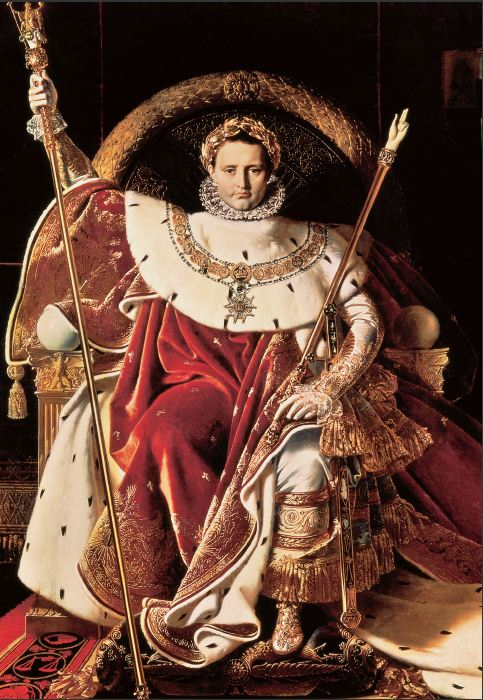
\includegraphics[width=\paperwidth]{napoleon}%

}


\cleardoublepage
\fullpageimage

\cxset{style16}
\chapter{Victorian England:\\ Introduction 16}
\label{style16}
This design from a Social Sciences book had to be set into two vboxes and negative skips allowed to line
up the numbers. Once I am totally happy with it, I will add parameter adjustments, as well as a bit of automation of length calculations.
\thispagestyle{empty}

\medskip

\begin{figure}[ht]
\centering
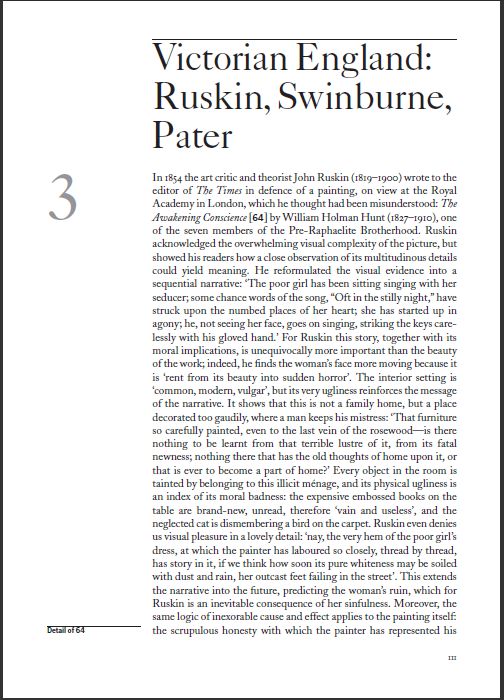
\includegraphics[width=0.35\textwidth]{./chapters/chapter16}
\end{figure}
\lipsum[2]

\cxset{geometry marginparsep/.code=\setlength\marginparsep{#1},
          geometry marginparwidth/.code=\setlength{\marginparwidth}{#1}}

\section{Technical notes}

This design looks simple but takes a bit of effort to achieve it, especially due to the tendency of LaTeX and the TeX engine to make decisions for you. Firstly we cannot reset the page geometry between the image and the chapter, as this will either result in unpredictable behaviour or if you use the \cs{newgeometry} macro, it will for certain leave a blank page in between.

\begin{description}
\item [image sizing] The image is set at \textbf{width=paperwidth}. This can vary depending on the page geometry and the image aspect ratio. In general you may need to ensure that your image has the same aspect ratio as the page to avoid problems with placement and the generation of extra blank pages.
\item [image caption] The image caption is placed using the picture environment, so that it can be typeset absolutely, feel free to use TikZ for the same purpose. We also use Heiko Oberdiek's the \pkg{picture} package to make calculations easier by specifying actual dimensions and not needing to strip the point.
\end{description}

% Best to always restore geometry after you have changed it.

\restoregeometry


%%%%%%%%%%%%%%%%%%%%%%%%%%%%%%%%%%%%%%%%%%%%
%%%%%%  STYLE 17
%%%%%%%%%%%%%%%%%%%%%%%%%%%%%%%%%%%%%%%%%%%
\newgeometry{left=7cm,right=2cm, marginparsep=15pt, marginparwidth=4.2cm,top=2cm,%
reversemarginpar}
\cxset{style17/.style={
 name={},
 numbering=arabic,
 number font-size=\huge,
 number font-family=\sffamily,
 number font-weight=\bfseries,
 number before=,
 number dot=.,
 number color=\color{purple},
 number after=\thinspace,
 number position=rightname,
 chapter font-family=\sffamily,
 chapter font-weight=\bfseries,
 chapter font-size=\LARGE,
 chapter before={\vspace*{20pt}\par\hfill},
 chapter after={},
 chapter color={black!90},
 title beforeskip={},
 title afterskip={\vspace*{70pt}\par},
 title before={},
 title after={},
 title font-family=\sffamily,
 title font-color=\color{purple},
 title font-shape=\upshape,
 title font-weight=\bfseries,
 title font-size=\huge,
 section numbering=none,
 section beforeskip=10pt,
 section afterskip=10pt,
 section font-family=\rmfamily,
 section font-shape=\slshape,
 geometry marginparwidth=4.5cm,
 geometry marginparsep=20pt}}
\cxset{style17}

\chapter{Introduction to Style Seventeen}

I tend to favour this design for books that have a lot of pictures. It brings the design into the margins and leaves plentiful white space in the margins. From a programming point of view the chapter is the opposite of openany. It has to open on an odd number.

\marginpar{%
\vspace*{0.2\textheight}
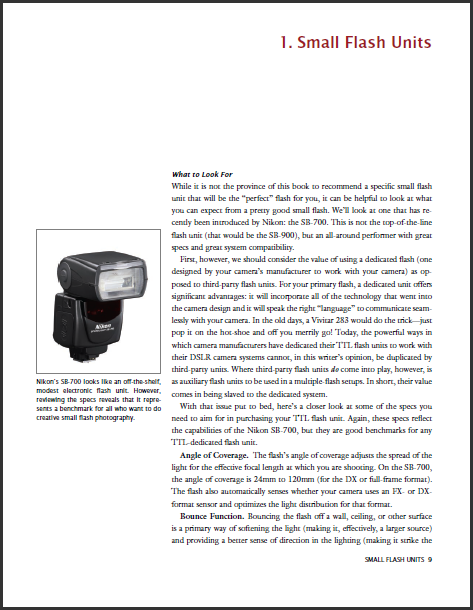
\includegraphics[width=\marginparwidth]{./chapters/chapter17}\par
{\footnotesize\lorem}
}

\section{Use the margins}

Adjustments to the geometry layout can be carried out temporarily or permanently via the use of keys and
the geometry package. These are probably the less problematic and easier to set geometry settings.

\section{Margin notes}

Marginal notes use the same mechanism as
floats to communicate with the \cs{output} routine. Marginal notes are distinguished from
floats by having a negative placement specification. The command
\cs{marginpar}\oarg{left text}\marg{right text} generates a marginal note in a parbox,
using LTEXT if it's on the left and RTEXT if it's on the right.
(Default is RTEXT = LTEXT.) It uses the following parameters.
\cs{marginparwidth}: Width of marginal notes.
\cs{marginparsep}: Distance between marginal note and text.
the page layout to determine how to move the marginal
note into the margin. E.g.,

\begin{tcolorbox}
\begin{lstlisting}
\@leftmarginskip ==\hskip -\marginparwidth \hskip -\marginparsep .
\end{lstlisting}
\end{tcolorbox}

\cs{marginparpush} Minimum vertical separation between \cs{marginpar}'s
Marginal notes are normally put on the outside of the page
if @mparswitch = true, and on the right if @mparswitch = false.
The command \cs{reversemarginpar} reverses the side where they
are put. \cs{normalmarginpar} undoes \cs{reversemarginpar}.
These commands have no effect for two-column output.
\marginpar{\footnotesize \textsc{\bfseries NOTE:} if two marginal notes appear on the same line of
text, then the second one could appear on the next page, in
a funny position.}
\section{Sample text}
\lipsum[2-4]

\restoregeometry

\restoregeometry

\cxset{
 name={CHAPTER},
 numbering=arabic,
 number font-size=\Large,
 number font-family=\rmfamily,
 number font-weight=\normalfont,
 number before=\kern0.5em,
 number after=\hfill\hfill\par\vspace*{20pt}\centerline{\decoone}\vspace*{20pt},
 number dot={},
 number position=rightname,
 name=CHAPTER,
 chapter font-family=rmfamily,
 chapter font-weight=mdweight,
 chapter font-size=Large,
 chapter before={\vspace*{20pt}\par\hfill},
 chapter after={},
 chapter color=black!90,
 number color=black!90,
 chapter title align=center,
 chapter title text-align=center,
 title margin-left=0pt,
 title margin bottom=50pt,
 title margin top=30pt,
 title before=,
 title after=,
 title font-family=rmfamily,
 title font-shape=upshape,
 title font-color= black!90,
 title font-weight=\normalfont,
 title font-size=Huge,
 title display=block}

\chapter[Style 18]{Chapter Style Eighteen}

\parindent0pt
This design introduces an ornament. There are a number of packages on ctan that provide ornaments. If you using XeLaTeX it is also possible to use system fonts. The ornament is introduced with the key number after. At this point also we introduced all the vertical skips.
\medskip
\begin{figure}[ht]
\centering
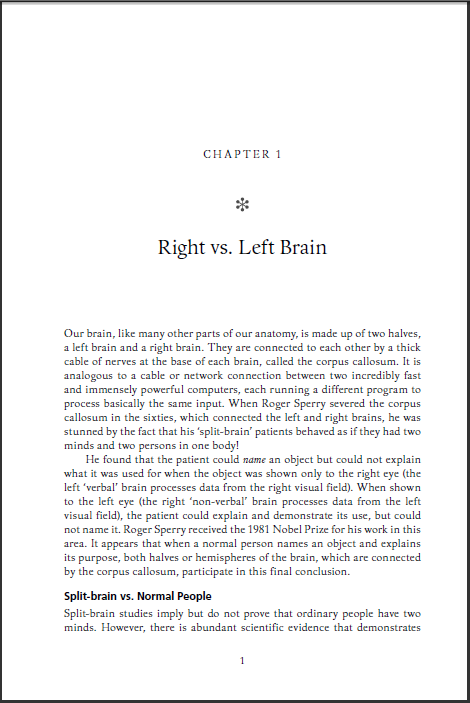
\includegraphics[width=0.45\textwidth]{./chapters/chapter18.png}
\end{figure}

\section{Sections}
\lorem

\subsection{Subsections}
\lorem


\subsubsection{Subsubsections}
\lorem

\parindent3em
\newcommand{\wb}[2]{\fontsize{#1}{#2}\usefont{U}{webo}{xl}{n}}
\newcommand{\showb}[1]{\wb{12}{14}#1}
\newfontfamily{\minion}{MinionPro-Regular.otf}
\def\ornament{{\minion \char"2740}}

\cxset{chapter name=,
          epigraph align=center,
          epigraph text align=center,
          epigraph rule width=0pt,
          title margin top=10pt,
          number font-size=small,
          number after=\hfill\hfill\par\vspace*{5pt}\centerline{\showb{[]}}\vspace*{5pt},
           %number after=\hfill\hfill\par\vspace*{5pt}\centerline{\Large\ornament}\vspace*{5pt},
          }
\chapter{THE IMPRESSIONISTS IN NEW YORK}


\epigraph{\ldots\itshape a pile of unsung treasures \ldots}{}
\minion

\lettrine{O}{n 13 March 1886, Paul Durant-Ruel and his young son Charles were travelling} through the streets of Paris, on their way to Gare Gare Saint-Lazare. In the two decades since Paul had
inherited his father’s business, Paris had been transformed. Haussmann had
realized his dream. The city was only three years away from the
Exposition of 1889 and the erection of the new Eiffel Tower, the symbol
of modern Paris. By 1890, Baron Haussmann would be saying of his newly
created capital of Europe, ‘these days, it’s fashionable to admire old Paris,
which people only know about from books’. Some areas of Paris had
hardly changed: the poor still lived in the shacks of Montmartre or the
shanties of Belleville; there were still cholera, typhoid, deaths in childbirth
and infant mortality. But to the uninitiated, those problems were now
hidden from view. Paris had a new image: the new Republic was
streamlined and stylish, the epitome of healthy living and good taste.
Haussmann’s Paris was architecturally modern, stratified by wealth,
quintessentially urban and, above all, commercially prosperous.

\begin{figure}[ht]
\centering
\fbox{%
\includegraphics[width=0.8\textwidth]{impressionist-lives}}
\caption{Spread from the Book \emph{The Private Lives of the Impressionists} by Sue Rose and published by Harper Collins.}
\end{figure}

The ctan repository has two good packages for ornamental fonts \pkgname{webomints} and \pkgname{fourier-orns}. The one shown in the orgininal publication is from Minion Symbols Pro.

They have been inserted in the template by using the |number after| key and a custom command from the \pkgname{webomints}
\bigskip

\begin{scriptexample}{}{}
\begin{verbatim}
\newcommand{\wb}[2]{\fontsize{#1}{#2}\usefont{U}{webo}{xl}{n}}
\newcommand{\showb}[1]{\wb{12}{14}#1}
\end{verbatim}
\end{scriptexample}


\ornament

\let\oldsection\section
\long\def\section{%
\par\medskip
\addvspace{20pt}
\centerline{{\LARGE *}}%
\addvspace{20pt}}


Cézanne wanted nothing to do with any war. Taking Hortense with him,
he left their garret at 53, rue Notre-Dame-des-Champs, and made for Aix.
Zola, who had recently married, returned to Provence with his wife,
heading from there to Marseilles. Monet, still in Trouville, waited for the
time being to see how events would turn out. Degas, Renoir, Bazille and
Manet, who stayed behind, were all eligible to fight

Cézanne had been working right up to the last minute to meet the 1866
Salon deadline. On the last possible day for submitting, a wheelbarrow
arrived outside the Palais de l’Industrie, pushed and pulled by Cézanne
and Oller, his Cuban friend from Suisse’s. Cézanne rushed to unwrap his
paintings, eager to show them to anyone who wanted to see. But by now
his hopes were not particularly high. When both his paintings were
rejected he was hardly surprised. He headed straight back to Aix,
complaining to Pissarro about the ‘rotten’ family he was being forced to
rejoin, all of them ‘boring beyond measure’. 

\section

Sections are marked with a single asterisk like ornament. This is a common element
in many non-fiction as well as fiction books. Some might have anything from on to three
asterisks. Many books printed in the nineteenth century have very fancy end section ornamentation.
I like the simplicity of the one asterisk.

\let\section\oldsection
\cxset{title display=in-line block}




\cxset{style19/.style={
 name={},
 numbering=arabic,
 number font-size=Huge,
 number font-family=rmfamily,
 number font-weight=bfseries,
 number before=\par\offinterlineskip,
 number after=\kern0.5em,
 number dot={ },
 number position=rightname,
 chapter font-family=rmfamily,
 chapter font-weight=mdseries,
 chapter font-size=Huge,
 chapter before=\par,
 chapter after=\par,
 chapter color=black!90,
 number  color=black!90,
 chapter title width=0.8\textwidth,
 chapter title align=left,
 title   beforeskip=,
% title afterskip={\vspace*{50pt}\par},
 title margin top=0pt,
 title margin bottom=50pt,
 title margin-left=0pt,
 title before=,
 title after=\par,
 chapter title text-align=left,
 title font-family=rmfamily,
 title font-color=black!90,
 title font-weight=bfseries,
 title font-size=Huge}}
 
\parindent1em

\cxset{style19}
\chapter{Introduction to chapter style nineteen}

I first visited the Gulf seven years after its independence. As Simon C. Smith puts it, in his book \emph{Britain’s Revival and Fall in the Gulf} the decolonization of the Gulf was a mere footnote on British history. As I have lived in and I am currently still working in the area in this footnote for about twelve years Smith’s book sheds light to the beginnings of the Gulf.

\medskip
\begin{figure}[ht]
\centering 
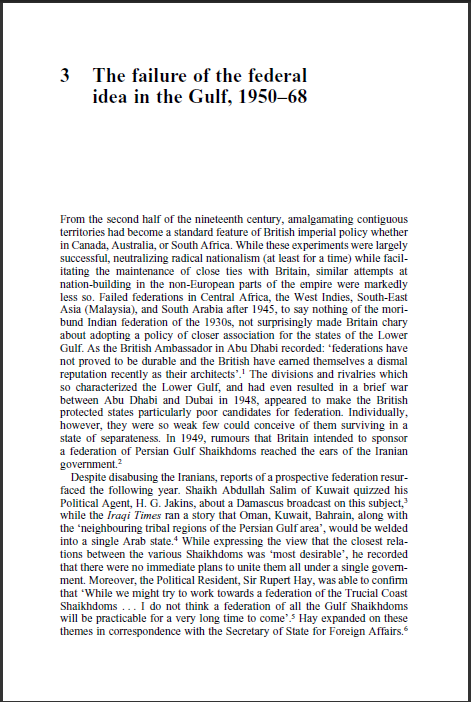
\includegraphics[width=0.5\textwidth]{./chapters/chapter19.png}
\end{figure}

The book’s typography is what one expects from an academic publication. The headings are simple and the text is typeset in Times Roman. I was tempted to name this template \emph{plain vanilla} but perhaps it deserves better.
There is a large section of book designers that believe that the typography of a book should be like a crystal glass.

\begin{quote}
Now the man who first chose glass instead of clay or metal to hold his wine was a ``modernist" in the sense in which I am going to use that term. That is, the first he asked of this particular object was not "How should it look?" but ``What must it do?" and to that extent all good typography is modernist.	
\end{quote}

Throughout the essay, Warde argues for the discipline and humility required to create quietly set, ``transparent" book pages.

Now, back to the template one of the difficulties we will face is that the chapter title blocks are set in Once we adjust the title to be anything less than the width of the text block, we will also need to be careful
about words in order to give it some balance.
two or three lines and they do not extend to the full length of the text block.

The main settings are as follows:

\begin{verbatim}
\cxset{reset,
 chapter title width=0.65\textwidth,
 chapter title align=raggedright,}
\end{verbatim}


\cxset{chapter opening=anywhere}
\chapter{The failure of the federal idea in the Gulf, 1950-68}

The book does not have any lower level headings. Another characteristic is a subtitle below the main chapter block on some of the chapters. The subtitle is set in normal weight and is \emph{partially} used as a heading. 

\testsections





<<<<<<< HEAD
\@specialfalse
%%%%%%%%%%%%%%%%%%%%%%%%%%%%%%%%%%%%%%%%%%%
%%%%%%  STYLE 21
%%%%%%%%%%%%%%%%%%%%%%%%%%%%%%%%%%%%%%%%%%%
\newgeometry{left=4.5cm,right=2.5cm, marginparsep=15pt, marginparwidth=4.2cm,top=2cm,%
reversemarginpar}
\cxset{
 chapter opening=right,
 name={},
 numbering=none,
 number font-size=\Large,
 number font-family=\rmfamily,
 number font-weight=\bfseries,
 number before=,
 number after=,
 number position=rightname,
 chapter font-family=\sffamily,
 chapter font-weight=\normalfont,
 chapter font-size=\Large,
 chapter before={\vspace*{0.3\textheight}},
 chapter after={\par},
 chapter color={black!90},
 number color=\color{black!90},
 title beforeskip={},
 title afterskip={\par\rule{\textwidth}{3.5pt}\vspace{20pt}},
 title before={},
 title after={},
 title font-family=\sffamily,
 title font-color=\color{black},
 title font-weight=\bfseries,
 title font-size=\Huge,
 author block=false}


\chapter{INTRODUCTION TO STYLE 21}

\lipsum[1]
\medskip
\begin{figure}[ht]
\centering
\fbox{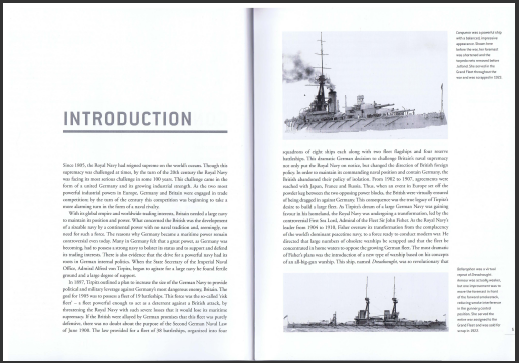
\includegraphics[width=0.65\textwidth]{./chapters/chapter21}}
\end{figure}
\lipsum[1]
\clearpage
=======
\@specialfalse
%%%%%%%%%%%%%%%%%%%%%%%%%%%%%%%%%%%%%%%%%%%
%%%%%%  STYLE 21
%%%%%%%%%%%%%%%%%%%%%%%%%%%%%%%%%%%%%%%%%%%
\newgeometry{left=4.5cm,right=2.5cm, marginparsep=15pt, marginparwidth=4.2cm,top=2cm,%
reversemarginpar}
\cxset{
 chapter opening=right,
 name={},
 numbering=none,
 number font-size=\Large,
 number font-family=\rmfamily,
 number font-weight=\bfseries,
 number before=,
 number after=,
 number position=rightname,
 chapter font-family=\sffamily,
 chapter font-weight=\normalfont,
 chapter font-size=\Large,
 chapter before={\vspace*{0.3\textheight}},
 chapter after={\par},
 chapter color={black!90},
 number color=\color{black!90},
 title beforeskip={},
 title afterskip={\par\rule{\textwidth}{3.5pt}\vspace{20pt}},
 title before={},
 title after={},
 title font-family=\sffamily,
 title font-color=\color{black},
 title font-weight=\bfseries,
 title font-size=\Huge,
 author block=false}


\chapter{INTRODUCTION TO STYLE 21}

\lipsum[1]
\medskip
\begin{figure}[ht]
\centering
\fbox{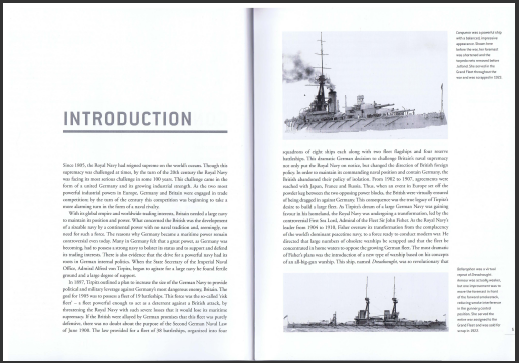
\includegraphics[width=0.65\textwidth]{./chapters/chapter21}}
\end{figure}
\lipsum[1]
\clearpage
>>>>>>> merged



\restoregeometry

\newgeometry{left=4.5cm,right=2.5cm, marginparsep=15pt, marginparwidth=4.2cm,top=2cm,
reversemarginpar}

\setdefaults
\cxset{style22/.style={
 name={},
 numbering=none,
 number font-size=\Large,
 number font-family=\rmfamily,
 number font-weight=\bfseries,
 number before=,
 number after=,
 number position=rightname,
 chapter font-family=\sffamily,
 chapter font-weight=\normalfont,
 chapter font-size=\Large,
 chapter before=\vspace*{-10pt},
 chapter after={},
 chapter color=black!90,
 number color= black!90,
 title beforeskip= \raggedleft,
 title afterskip={\vspace{70pt}},
 title before=\hspace*{-2cm},
 title after={},
 title font-family=\sffamily,
 title font-color=black,
 title font-weight=\bfseries,
 title font-size=\huge,
 section numbering=none,
 section font-family=\sffamily,
 section font-weight=\bfseries,
 section color=black,
 section indent= 10pt,
 subsection indent = 0pt,
 header style=plain}}


\cxset{style22}
\renewsection\renewsubsection

\chapter{INTRODUCTION TO STYLE TWENTY TWO}\index{style22}\index{lettrine}\index{drop cap}

\section{INTRODUCTION}

\renewcommand{\DefaultLoversize}{0.3}
\renewcommand{\LettrineTextFont}{\fontfamily{Minion Pro}\normalfont\itshape}
\renewcommand{\LettrineFontHook}{%
\fontseries{bx}\fontshape{up}\color{gray}}

\cxset{lettrine lines/.code=\global\setcounter{DefaultLines}{#1}}

\cxset{lettrine lines=5}

\lettrine[lraise=0.0, nindent=0em, slope=-.5em]{Y}{oic} \lipsum[1]

\medskip
\begin{figure}[ht]
\centering
\fbox{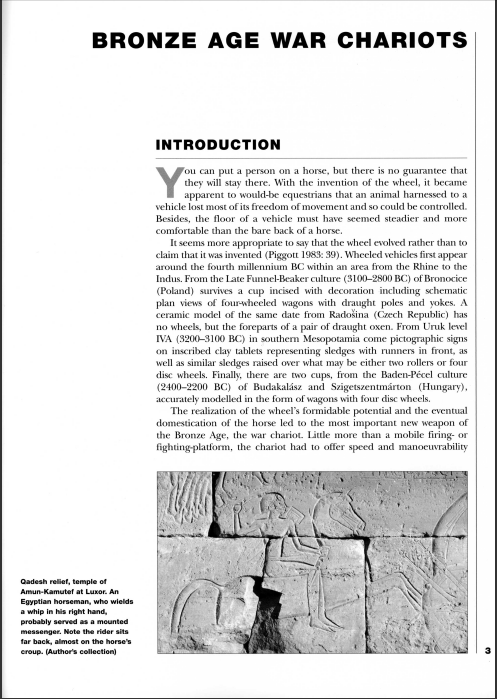
\includegraphics[width=0.5\textwidth]{./chapters/chapter22.png}}
\end{figure}

\lipsum[1-2]
\parindent0pt

\cxset{toc image=false},

\long\gdef\versochapter#1{%
  \vspace*{3cm}
  \minipage{\textwidth}
  \hfill\includegraphics[width=0.63\textwidth]{\chapterimage@cx}\par
  \vspace*{6pt}
  \hfill\minipage{0.75\textwidth}
  {\HUGE\bfseries\flushright #1\endflushright}
  \endminipage
  \endminipage
  \newpage


\vspace*{10cm}
\@specialfalse
\@openleftfalse
\@openanyfalse
\@openrighttrue
}


\newgeometry{bottom=2.5cm}

\cxset{
   chapter image/.code={\def\chapterimage@cx{#1}},
   chapter opening/.is choice,
   chapter opening/verso/.code={\@specialtrue\@openlefttrue
   \gdef\customdesign@cx##1{\versochapter{##1}}}
}

\cxset{
 chapter image=onesowndeath,
 chapter opening=verso,
 name={},
 numbering=none,
 number font-size=\LARGE,
 number font-family=\rmfamily,
 number font-weight=\bfseries,
 number before=,
 number dot=,
 number after=,
 number position=leftname,
 chapter font-family=\sffamily,
 chapter font-weight=\normalfont,
 chapter font-size=\Large,
 chapter before={\vspace*{0pt}\par},
 chapter after={\hfill\hfill\par},
 chapter color={black!90},
 number color=\color{purple},
 title beforeskip={\vspace*{0pt}},
 title afterskip={\vspace*{0.4\textheight}\par},
 title before={},
 title after={},
 title font-family=\sffamily,
 title font-color=\color{purple},
 title font-weight=\bfseries,
 title font-size=\LARGE,
 header style=plain,
 pagestyle=plain,
 }

\@specialtrue

\chapter[VERSO CHAPTERS]{Verso Chapters}

\parindent1.5em
{\HUGE V}erso chapter openings are not common. One design that I found quite attractive is \lipsum[1-3] \textit{From Western attitudes toward death from the middle ages to the present}, Philippe Ari\'es. London, 1974.

\begin{figure}
\includegraphics[width=\textwidth]{versochapter01}
\caption{Chapter opening on verso page.}
\end{figure}


\newfontfamily{\neutra}{NeutraText-Bold.otf}
\newfontfamily{\vijaya}{Vijaya-Bold.ttf}
\parindent3em
\cxset{style26/.style={%
 chapter opening=any,
 name=Chapter,
 numbering=arabic,
 number font-size=LARGE,
 number font-family=rmfamily,
 number font-weight=itshape,
 number before=\kern1.5em,
 number position=rightname,
 chapter font-family=itshape,
 chapter font-weight=rmfamily,
 chapter font-size=LARGE,
 number display=inline,
 number float=left,
 number after=\vbox{\hrule width\textwidth height1pt depth0pt\vskip1.5pt% 
                       \hrule width\textwidth height3pt depth0pt},
 chapter display=block,
 chapter float=left,
 chapter before={},
 chapter after=,
 chapter color= black!90,
 chapter afterindent=true,
 number color= black!90,
 title before=,
 title after=,
 title margin top=30pt,
 title margin bottom=30pt,
 title font-family=neutra,
 title font-color= black!80,
 title font-weight=bfseries,
 title font-size=huge,
 title spaceout=none,
 chapter title align=center,
 chapter title width=\textwidth,
 author block=false,
 section font-family=vijaya,
 section font-size=LARGE,
 section numbering=none,
 section afterindent=false,
 subsection numbering=none,
 subsection font-family=vijaya,
 subsection color=black,
 subsection font-size=LARGE%
 }}



%%%%%%%%%%%%%%%%%%%%%%%%%%%%%%%%%%%%%%%%%%%
%%%%%%  STYLE 27
%%%%%%%%%%%%%%%%%%%%%%%%%%%%%%%%%%%%%%%%%%%

\cxset{
 author block=false,
 name={},
 numbering=arabic,
 number font-size=\HUGE,
 number font-family=\sffamily,
 number font-weight=\bfseries,
 number before={},
 number dot=,
 number position=leftname,
 chapter font-family=\sffamily,
 chapter font-weight=\normalfont,
 chapter font-size=\small,
 number after={},
 chapter before={\vspace*{50pt}},
 chapter after={\par\vskip12pt},
 chapter color={black!90},
 number color=\color{black!90},
 title beforeskip={},
 title afterskip={\vspace{30pt}},
 title before=,
 title after={\par},
 title font-family=\sffamily,
 title font-color=\color{black!80},
 title font-weight=\bfseries,
 title font-size=\huge}
\chapter{Introduction to style twenty seven Dr. Yiannis Lazarides and Athena Lazarides}
\lipsum[3]

\medskip
\begin{figure}[ht]
\centering
\fbox{\includegraphics[width=0.5\textwidth]{./chapters/chapter27}}
\end{figure}
\lipsum[2-3]


%%%%%%%%%%%%%%%%%%%%%%%%%%%%%%%%%%%%%%%%%%%
%%%%%%  STYLE 28
%%%%%%%%%%%%%%%%%%%%%%%%%%%%%%%%%%%%%%%%%%%

\cxset{
 name={},
 numbering=arabic,
 number font-size=\HUGE,
 number font-family=\sffamily,
 number font-weight=\bfseries,
 number before={},
 number position=leftname,
 chapter font-family=\sffamily,
 chapter font-weight=\normalfont,
 chapter font-size=\small,
 number after={},
 chapter before={},
 chapter after={\hspace*{20pt}},
 chapter color={black!90},
 number color=\color{black!90},
 title beforeskip={},
 title afterskip={\vspace{70pt}},
 title before=,
 title after={\par},
 title font-family=\itshape,
 title font-color=\color{black!80},
 title font-weight=\itshape,
 title font-size=\LARGE}
\chapter{Introduction to Style Twenty Eight}

The interesting part of this style is that it uses roman numerals to display the counter that is in a different font than that used for the chapter name.
\medskip
\begin{figure}[ht]
\centering
\includegraphics[width=0.6\textwidth]{./chapters/chapter28}
\end{figure}
\lipsum[2]

<<<<<<< HEAD
%%%%%%%%%%%%%%%%%%%%%%%%%%%%%%%%%%%%%%%%%%%
%%%%%%  STYLE 29
%%%%%%%%%%%%%%%%%%%%%%%%%%%%%%%%%%%%%%%%%%%
 \cxset{style29/.style={
 name={},
 numbering=arabic,
 number font-size=\normalsize,
 number font-family=\sffamily,
 number font-weight=\bfseries,
 number before={\vspace*{50pt}},
 number position=leftname,
 number after=\vskip-7.5pt,
 chapter font-family=\sffamily,
 chapter font-weight=,
 chapter font-size=\small,
 chapter before={\vskip2.5pt},
 chapter after={\thinrule\par},
 chapter color={black!90},
 number color=\color{black!90},
 title beforeskip={},
 title afterskip={\bigskip},
 title before=,
 title after={\par},
 title font-family=\rmfamily,
 title font-color=\color{black!80},
 title font-weight=\bfseries,
 title font-size=\huge},
 section indent=0pt,
 section font-family=\rmfamily,
 section font-shape=\upshape}
\cxset{style29}

\chapter{Introduction to Style Twenty Nine}
\bigskip\bigskip

\textit{Lambert Schoemacher}
\bigskip\bigskip\bigskip\bigskip

\section{Introduction}
The interesting part of this style is that it uses roman numerals to display the counter that is in a different font than that used for the chapter name.
\medskip

\begin{figure}[ht]
\centering
\includegraphics[width=0.6\textwidth]{./chapters/chapter29}
\end{figure}
\lipsum[3]

=======
%%%%%%%%%%%%%%%%%%%%%%%%%%%%%%%%%%%%%%%%%%%
%%%%%%  STYLE 29
%%%%%%%%%%%%%%%%%%%%%%%%%%%%%%%%%%%%%%%%%%%
 \cxset{style29/.style={
 name={},
 numbering=arabic,
 number font-size=\normalsize,
 number font-family=\sffamily,
 number font-weight=\bfseries,
 number before={\vspace*{50pt}},
 number position=leftname,
 number after=\vskip-7.5pt,
 chapter font-family=\sffamily,
 chapter font-weight=,
 chapter font-size=\small,
 chapter before={\vskip2.5pt},
 chapter after={\thinrule\par},
 chapter color={black!90},
 number color=\color{black!90},
 title beforeskip={},
 title afterskip={\bigskip},
 title before=,
 title after={\par},
 title font-family=\rmfamily,
 title font-color=\color{black!80},
 title font-weight=\bfseries,
 title font-size=\huge},
 section indent=0pt,
 section font-family=\rmfamily,
 section font-shape=\upshape}
\cxset{style29}

\chapter{Introduction to Style Twenty Nine}
\bigskip\bigskip

\textit{Lambert Schoemacher}
\bigskip\bigskip\bigskip\bigskip

\section{Introduction}
The interesting part of this style is that it uses roman numerals to display the counter that is in a different font than that used for the chapter name.
\medskip

\begin{figure}[ht]
\centering
\includegraphics[width=0.6\textwidth]{./chapters/chapter29}
\end{figure}
\lipsum[3]

>>>>>>> merged

<<<<<<< HEAD
%%%%%%%%%%%%%%%%%%%%%%%%%%%%%%%%%%%%%%%%%%%
%%%%%%  STYLE 30
%%%%%%%%%%%%%%%%%%%%%%%%%%%%%%%%%%%%%%%%%%%

\cxset{style30/.style={
 name={},
 numbering=arabic,
 number font-size=\HUGE,
 number font-family=\sffamily,
 number font-weight=\bfseries,
 number before={\rule{\textwidth}{5pt}\par\vspace*{12pt}\hspace*{20pt}\minipage{1cm}\vspace*{8pt}},
 number after=\endminipage\hspace{1em},
 number position=leftname,
 chapter font-family=\sffamily,
 chapter font-weight=\normalfont,
 chapter font-size=\small,
 chapter before={},
 chapter after={\hspace*{20pt}},
 chapter color={black!90},
 number color=\color{black!90},
 title beforeskip={},
 title afterskip={\vspace{30pt}},
 title before=\minipage[t]{10cm},
 title after={\endminipage\par},
 title font-family=\sffamily,
 title font-color=\color{black!80},
 title font-weight=\normalfont\sffamily,
 title font-size=\Huge}}

\cxset{style30}
\chapter{Introduction to Style Thirty\\ with a Somehow Long Title \\to Illustrate the Example}

Since we do not know how long a chapter title can end up, it is best to
typeset this using two minipages or parboxes. The number is pushed down slightly although it can look as good with both the number and the text fully aligned on top.
\medskip
\begin{figure}[ht]
\centering
\includegraphics[width=0.6\textwidth]{./chapters/chapter30}
\end{figure}
=======
%%%%%%%%%%%%%%%%%%%%%%%%%%%%%%%%%%%%%%%%%%%
%%%%%%  STYLE 30
%%%%%%%%%%%%%%%%%%%%%%%%%%%%%%%%%%%%%%%%%%%

\cxset{style30/.style={
 name={},
 numbering=arabic,
 number font-size=\HUGE,
 number font-family=\sffamily,
 number font-weight=\bfseries,
 number before={\rule{\textwidth}{5pt}\par\vspace*{12pt}\hspace*{20pt}\minipage{1cm}\vspace*{8pt}},
 number after=\endminipage\hspace{1em},
 number position=leftname,
 chapter font-family=\sffamily,
 chapter font-weight=\normalfont,
 chapter font-size=\small,
 chapter before={},
 chapter after={\hspace*{20pt}},
 chapter color={black!90},
 number color=\color{black!90},
 title beforeskip={},
 title afterskip={\vspace{30pt}},
 title before=\minipage[t]{10cm},
 title after={\endminipage\par},
 title font-family=\sffamily,
 title font-color=\color{black!80},
 title font-weight=\normalfont\sffamily,
 title font-size=\Huge}}

\cxset{style30}
\chapter{Introduction to Style Thirty\\ with a Somehow Long Title \\to Illustrate the Example}

Since we do not know how long a chapter title can end up, it is best to
typeset this using two minipages or parboxes. The number is pushed down slightly although it can look as good with both the number and the text fully aligned on top.
\medskip
\begin{figure}[ht]
\centering
\includegraphics[width=0.6\textwidth]{./chapters/chapter30}
\end{figure}
>>>>>>> merged



%%%%%%%%%%%%%%%%%%%%%%%%%%%%%%%%%%%%%%%%%%%
%%%%%%  STYLE 31
%%%%%%%%%%%%%%%%%%%%%%%%%%%%%%%%%%%%%%%%%%%

\cxset{style31/.style={
 name={},
 numbering=arabic,
 number font-size=\HUGE,
 number font-family=\sffamily,
 number font-weight=\bfseries,
 number before=,
 number after={},
 number position=leftname,
 chapter font-family=\sffamily,
 chapter font-weight=\normalfont,
 chapter font-size=\small,
 chapter before={},
 chapter after={\vskip2.5pt{\color{gray}\rule{3cm}{5pt}\rule[3.5pt]{\dimexpr\textwidth-3cm\relax}{0.4pt}}\par},
 chapter color={gray},
 number color=\color{gray},
 title beforeskip={},
 title afterskip={\vspace{30pt}},
 title before=,
 title after={\par{\color{gray}\rule[6pt]{3cm}{0.4pt}}\par},
 title font-family=\itshape,
 title font-color=\color{black},
 title font-weight=\itshape,
 title font-size=\LARGE}}

\cxset{style31}
\chapter{The Evolution of Organizations\\ and the Environment}

This is an unusual design by all counts. I did soften the rules a bit to make them a bit less conspicuous.
\medskip
\begin{figure}[ht]
\centering
\includegraphics[width=0.6\textwidth]{./chapters/chapter31}
\end{figure}

\lipsum[1-2]



\newgeometry{left=5cm,right=2cm,bottom=2cm}
\cxset{style32/.style={
 name=,
 numbering=arabic,
 number font-size=HHUGE,
 number font-family=sffamily,
 number font-weight=bfseries,
 number before={\hspace*{-60pt}},
 number position=leftname,
 number after={.},
 chapter font-family=sffamily,
 chapter font-weight=\normalfont,
 chapter font-size=\small,
 chapter before={\vspace*{50pt}\par\hspace*{-60pt}},
 chapter after={\hspace*{20pt}},
 chapter color=black!90,
 number color=black!90,
 title beforeskip={},
 title afterskip={\vspace{70pt}},
 title before=,
 title after=,
 chapter title align=left,
 title font-family=\itshape,
 title font-color=black!80,
 title font-weight=\bfseries,
 title font-shape=\itshape,
 title font-size= Huge,
}}

\cxset{style32}
\chapter{Introduction to Style Thirty Two}

This style has a modern look to it. Its main characteristic is the large chapter number and the fact that it is drawn into the margin. This is a common style used for computer books.
\medskip
\begin{figure}[ht]
\centering
\includegraphics[width=0.6\textwidth]{./chapters/chapter32.png}
\end{figure}
The example is from Python NLP book.



\restoregeometry
\cxset{style33/.style={
 name=CHAPTER,
 numbering=arabic,
 number font-size= LARGE,
 number font-family= rmfamily,
 number font-weight= \normalfont,
 number before={\par\hfill},
 number after={\hfill\hfill\par},
 number position=leftname,
 name=,
 chapter font-family=sffamily,
 chapter font-weight=normalfont,
 chapter font-size=\small,
 chapter before={\vskip10pt},
 chapter after={\vskip10pt\par},
 chapter color= black!90,
 number color= black!90,
 title beforeskip={},
% title afterskip={\vspace{50pt}},
 title margin bottom=6cm,
 title before=,
 title after=,
 chapter title align=center,
 title font-family=normalfont,
 title font-color= black!80,
 title font-weight=normalfont,
 title font-shape=upshape,
 title font-size=LARGE,
 section numbering=none,
 section font-size=Large,
 section align= center,
 section color=black!80}}

\cxset{style33}
\chapter{Introduction to Style Thirty Three}

The interesting part of this style is that it uses roman numerals to display the counter that is in a different font than that used for the chapter name.
\medskip
\begin{figure}[ht]
\centering
\includegraphics[width=0.6\textwidth]{./chapters/chapter33.png}
\end{figure}





%%%%%%%%%%%%%%%%%%%%%%%%%%%%%%%%%%%%%%%%%%%
%%%%%%  STYLE 34
%%%%%%%%%%%%%%%%%%%%%%%%%%%%%%%%%%%%%%%%%%%

\cxset{
 name=CHAPTER,
 numbering=Roman,
 number font-size=\small,
 number font-family=\rmfamily,
 number font-weight=\normalfont,
 number before={},
 number position=rightname,
 chapter font-family=\sffamily,
 chapter font-weight=\normalfont,
 chapter font-size=\small,
 number after={},
 chapter before={},
 chapter after={\par},
 chapter color={black!90},
 number color=\color{black!90},
 title beforeskip={},
 title afterskip={\vspace{50pt}},
 title before=,
 title after={\par},
 title font-family=\normalfont,
 title font-color=\color{black!80},
 title font-weight=\normalfont,
 title font-size=\LARGE}

\section{Basic astronomical phenomena}

The interesting part of this style is that it uses roman numerals to display the counter that is in a different font than that used for the chapter name.
\medskip
\begin{figure}[ht]
\centering
\includegraphics[width=0.6\textwidth]{./chapters/chapter34}
\end{figure}


\cxset{%
 name=CHAPTER,
 numbering=Roman,
 number font-size=\small,
 number font-family=\rmfamily,
 number font-weight=\normalfont,
 number before={},
 number position=rightname,
 chapter font-family=\sffamily,
 chapter font-weight=\normalfont,
 chapter font-size=\small,
 number after={},
 chapter before={},
 chapter after={\par},
 chapter color= black!90,
 number color= black!90,
 title beforeskip={},
 title afterskip={\vspace{50pt}},
 title before=,
 title after={\par},
 title font-family=\normalfont,
 title font-color=black!80,
 title font-weight=\normalfont,
 title font-size=\LARGE}
\chapter{Introduction to Style Thirty Five}

The interesting part of this style is that it uses roman numerals to display the counter that is in a different font than that used for the chapter name.
\medskip

\begin{figure}[ht]
\centering
\includegraphics[width=0.6\textwidth]{./chapters/chapter35}
\end{figure}



%%%%%%%%%%%%%%%%%%%%%%%%%%%%%%%%%%%%%%%%%%%
%%%%%%  STYLE 36
%%%%%%%%%%%%%%%%%%%%%%%%%%%%%%%%%%%%%%%%%%%

\cxset{numbering=none}
%% has errors
\cxset{style36/.style={
 name={},
 numbering={none},
 number font-size=\small,
 number font-family=\rmfamily,
 number font-weight=\normalfont,
 number before={},
 number position=rightname,
 chapter font-family=\sffamily,
 chapter font-weight=\normalfont,
 chapter font-size=\small,
 number after={},
 chapter before={},
 chapter after={},
 chapter color={black!90},
 number color=\color{black!90},
 title beforeskip={},
 title before=,
 title after={\vskip-12.5pt\rule{\columnwidth}{3.5pt}\vspace*{50pt}},
 title afterskip={},
 title font-family=\sffamily,
 title font-color=\color{black!80},
 title font-weight=\bfseries,
 title font-size=\Huge}}

\cxset{style36}
\chapter{Introduction to Style Thirty Six}

The interesting part of this style is that it uses roman numerals to display the counter that is in a different font than that used for the chapter name.
\medskip

\begin{figure}[ht]
\centering
\includegraphics[width=0.6\textwidth]{./chapters/chapter36}
\end{figure}

<<<<<<< HEAD

%%%%%%%%%%%%%%%%%%%%%%%%%%%%%%%%%%%%%%%%%%%
%%%%%%  STYLE 37
%%%%%%%%%%%%%%%%%%%%%%%%%%%%%%%%%%%%%%%%%%%

\cxset{style37/.style={
 name=CHAPTER,
 numbering=Roman,
 number font-size=\small,
 number font-family=\rmfamily,
 number font-weight=\normalfont,
 number before={},
 number position=rightname,
 chapter font-family=\sffamily,
 chapter font-weight=\normalfont,
 chapter font-size=\small,
 chapter spaceout=soul,
 number after={},
 chapter before={},
 chapter after={\par},
 chapter color={black!90},
 number color=\color{black!90},
 title beforeskip={},
 title afterskip={\vspace{50pt}},
 title before=,
 title after={\par},
 title font-family=\normalfont,
 title font-color=\color{black!80},
 title font-weight=\bfseries,
 title font-size=\huge}}

\cxset{style37}
\chapter{Introduction to Style Thirty Seven}

The interesting part of this style is that it uses roman numerals to display the counter that is in a different font than that used for the chapter name.
\medskip

\begin{figure}[ht]
\centering
\includegraphics[width=0.6\textwidth]{./chapters/chapter37}
\end{figure}

=======

%%%%%%%%%%%%%%%%%%%%%%%%%%%%%%%%%%%%%%%%%%%
%%%%%%  STYLE 37
%%%%%%%%%%%%%%%%%%%%%%%%%%%%%%%%%%%%%%%%%%%

\cxset{style37/.style={
 name=CHAPTER,
 numbering=Roman,
 number font-size=\small,
 number font-family=\rmfamily,
 number font-weight=\normalfont,
 number before={},
 number position=rightname,
 chapter font-family=\sffamily,
 chapter font-weight=\normalfont,
 chapter font-size=\small,
 chapter spaceout=soul,
 number after={},
 chapter before={},
 chapter after={\par},
 chapter color={black!90},
 number color=\color{black!90},
 title beforeskip={},
 title afterskip={\vspace{50pt}},
 title before=,
 title after={\par},
 title font-family=\normalfont,
 title font-color=\color{black!80},
 title font-weight=\bfseries,
 title font-size=\huge}}

\cxset{style37}
\chapter{Introduction to Style Thirty Seven}

The interesting part of this style is that it uses roman numerals to display the counter that is in a different font than that used for the chapter name.
\medskip

\begin{figure}[ht]
\centering
\includegraphics[width=0.6\textwidth]{./chapters/chapter37}
\end{figure}

>>>>>>> merged

<<<<<<< HEAD


%%%%%%%%%%%%%%%%%%%%%%%%%%%%%%%%%%%%%%%%%%%
%%%%%%  STYLE 38
%%%%%%%%%%%%%%%%%%%%%%%%%%%%%%%%%%%%%%%%%%%

\cxset{style38/.style={
 name=,
 numbering=arabic,
 number font-size=\huge,
 number font-family=\rmfamily,
 number font-weight=\normalfont,
 number before={\begin{center}},
 number position=leftname,
 chapter font-family=\sffamily,
 chapter font-weight=\normalfont,
 number after={\vspace*{6.5pt}\par},
 chapter before={},
 chapter after={},
 chapter color={black!90},
 number color=\color{black!90},
 title beforeskip={},
 title afterskip={\vspace{50pt}},
 title before=,
 title after={\par\end{center}} ,
 title font-family=\rmfamily,
 title font-color=\color{black!80},
 title font-weight=\normalfont,
 title font-size=\huge,
 chapter font-size=,
}}

\cxset{style38,
       author block=true,
       author block format=\centering}
\chapter{STAGES OF INITIATION IN THE\\ ELEUSINIAN AND\\ SAMOTHRACIAN MYSTERIES\\STYLE 38}

This style uses rules to enclose both the chapter name and number as well as the title, which necessarily needs to be rather short.
\medskip

\begin{figure}[ht]
\centering
\includegraphics[width=0.6\textwidth]{./chapters/chapter38}
\end{figure}

=======


%%%%%%%%%%%%%%%%%%%%%%%%%%%%%%%%%%%%%%%%%%%
%%%%%%  STYLE 38
%%%%%%%%%%%%%%%%%%%%%%%%%%%%%%%%%%%%%%%%%%%

\cxset{style38/.style={
 name=,
 numbering=arabic,
 number font-size=\huge,
 number font-family=\rmfamily,
 number font-weight=\normalfont,
 number before={\begin{center}},
 number position=leftname,
 chapter font-family=\sffamily,
 chapter font-weight=\normalfont,
 number after={\vspace*{6.5pt}\par},
 chapter before={},
 chapter after={},
 chapter color={black!90},
 number color=\color{black!90},
 title beforeskip={},
 title afterskip={\vspace{50pt}},
 title before=,
 title after={\par\end{center}} ,
 title font-family=\rmfamily,
 title font-color=\color{black!80},
 title font-weight=\normalfont,
 title font-size=\huge,
 chapter font-size=,
}}

\cxset{style38,
       author block=true,
       author block format=\centering}
\chapter{STAGES OF INITIATION IN THE\\ ELEUSINIAN AND\\ SAMOTHRACIAN MYSTERIES\\STYLE 38}

This style uses rules to enclose both the chapter name and number as well as the title, which necessarily needs to be rather short.
\medskip

\begin{figure}[ht]
\centering
\includegraphics[width=0.6\textwidth]{./chapters/chapter38}
\end{figure}

>>>>>>> merged

<<<<<<< HEAD



%%%%%%%%%%%%%%%%%%%%%%%%%%%%%%%%%%%%%%%%%%%
%%%%%%  STYLE 39
%%%%%%%%%%%%%%%%%%%%%%%%%%%%%%%%%%%%%%%%%%%

\cxset{
 name=CHAPTER,
 numbering=arabic,
 number font-size=\LARGE,
 number font-family=\sffamily,
 number font-weight=\bfseries,
 number before={},
 number position=rightname,
 chapter font-family=\sffamily,
 chapter font-weight=\bfseries,
 number after={},
 chapter before={\rule{\textwidth}{2pt}\par},
 chapter after={\vskip0pt\vspace*{-8pt}\rule{\textwidth}{.4pt}\vskip-7pt},
 chapter color={black!90},
 number color=\color{black!90},
 title beforeskip={},
 title afterskip={\vspace{50pt}},
 title before=,
 title after={\par\vskip-16.5pt\rule{\textwidth}{0.4pt}\par} ,
 title font-family=\sffamily,
 title font-color=\color{black!80},
 title font-weight=\bfseries,
 title font-size=\LARGE,
 chapter font-size=\LARGE,
 author block=false}

\chapter{STYLE 39}

This style uses rules to enclose both the chapter name and number as well as the title, which necessarily needs to be rather short.
\medskip

\begin{figure}[ht]
\centering
\includegraphics[width=0.6\textwidth]{./chapters/chapter39}
\end{figure}
In the picture it does not look very attractive, but in the actual book it does. My observation is that the rule clearances are a bit tight and if you use this type of layout it is better to experiment until you get them right.

\begin{tcblisting}{}
\@makechapterhead[
 name=CHAPTER,
 numbering=arabic,
 number font-size=\LARGE,
 number font-family=\sffamily,
 number font-weight=\bfseries,
 number before={},
 number position=rightname,
 chapter font-family=\sffamily,
 chapter font-weight=\bfseries,
 number after={},
 chapter before={\rule{\textwidth}{2pt}\par},
 chapter after={\vskip0pt\vspace*{-8pt}\rule{\textwidth}{.4pt}\vskip-7pt},
 chapter color={black!90},
 number color=\color{black!90},
 title beforeskip={},
 title afterskip={\vspace{50pt}},
 title before=,
 title after={\par\vskip-19pt\rule{\textwidth}{0.4pt}\par} ,
 title font-family=\sffamily,
 title font-color=\color{black!80},
 title font-weight=\bfseries,
 title font-size=\LARGE,
 chapter font-size=\LARGE]{INTRODUCTION}
\end{tcblisting}

=======



%%%%%%%%%%%%%%%%%%%%%%%%%%%%%%%%%%%%%%%%%%%
%%%%%%  STYLE 39
%%%%%%%%%%%%%%%%%%%%%%%%%%%%%%%%%%%%%%%%%%%

\cxset{
 name=CHAPTER,
 numbering=arabic,
 number font-size=\LARGE,
 number font-family=\sffamily,
 number font-weight=\bfseries,
 number before={},
 number position=rightname,
 chapter font-family=\sffamily,
 chapter font-weight=\bfseries,
 number after={},
 chapter before={\rule{\textwidth}{2pt}\par},
 chapter after={\vskip0pt\vspace*{-8pt}\rule{\textwidth}{.4pt}\vskip-7pt},
 chapter color={black!90},
 number color=\color{black!90},
 title beforeskip={},
 title afterskip={\vspace{50pt}},
 title before=,
 title after={\par\vskip-16.5pt\rule{\textwidth}{0.4pt}\par} ,
 title font-family=\sffamily,
 title font-color=\color{black!80},
 title font-weight=\bfseries,
 title font-size=\LARGE,
 chapter font-size=\LARGE,
 author block=false}

\chapter{STYLE 39}

This style uses rules to enclose both the chapter name and number as well as the title, which necessarily needs to be rather short.
\medskip

\begin{figure}[ht]
\centering
\includegraphics[width=0.6\textwidth]{./chapters/chapter39}
\end{figure}
In the picture it does not look very attractive, but in the actual book it does. My observation is that the rule clearances are a bit tight and if you use this type of layout it is better to experiment until you get them right.

\begin{tcblisting}{}
\@makechapterhead[
 name=CHAPTER,
 numbering=arabic,
 number font-size=\LARGE,
 number font-family=\sffamily,
 number font-weight=\bfseries,
 number before={},
 number position=rightname,
 chapter font-family=\sffamily,
 chapter font-weight=\bfseries,
 number after={},
 chapter before={\rule{\textwidth}{2pt}\par},
 chapter after={\vskip0pt\vspace*{-8pt}\rule{\textwidth}{.4pt}\vskip-7pt},
 chapter color={black!90},
 number color=\color{black!90},
 title beforeskip={},
 title afterskip={\vspace{50pt}},
 title before=,
 title after={\par\vskip-19pt\rule{\textwidth}{0.4pt}\par} ,
 title font-family=\sffamily,
 title font-color=\color{black!80},
 title font-weight=\bfseries,
 title font-size=\LARGE,
 chapter font-size=\LARGE]{INTRODUCTION}
\end{tcblisting}

>>>>>>> merged

\cxset{
 name=,
 numbering=arabic,
 number font-size = LARGE,
 number font-family = sffamily,
 number font-weight = bfseries,
 number before={},
 number position=rightname,
 chapter font-family= sffamily,
 chapter font-weight= bfseries,
 chapter before=\hfill,
 number after=,
 chapter after=\hfill\hfill\vskip0pt ,
 chapter color = black!90,
 number color = black!90,
 title beforeskip=,
 title before=\begin{center},
 title after=\end{center},
 title font-family = sffamily,
 title font-color= black!80,
 title font-weight= bfseries,
 title font-size= LARGE,
 chapter font-size= LARGE,
 author block=true,
 author block format=\Large\begin{center},
 author names=Karin Wahl-Jorgensen and Thomas Hanitzch\end{center}}


\chapter{Introduction: On Why and How to Use Chapter Style Forty}

\label{ch:style40}

A simple design for sombre multi-author books. This type of design is now common in many publications such as proceedings, conferences and the like. They are actually mostly collections of articles, but formatted as books. The style comes with many variants.

\begin{figure}[ht]
\centering
\includegraphics[width=0.6\textwidth]{./chapters/chapter40.png}
\end{figure}

One issue with such designs is how to make it easy for the user to add the author block. There are two pathways, the one is to use \cs{cxset} and the other is to make a special command for it. The Chapter \nameref{ch:style40} presents difficulties in so far as we need to format the title in a more detailed manner.


%\makeatletter
\cxset{chapter author/.store in=\chapterauthor@cx}
\cxset{style41/.style={
 color=purple,
 name=CHAPTER,
 numbering=WORDS,
 number font-size=\large,
 number font-family=\rmfamily,
 number font-weight=\normalfont,
 number before={},
 number position=rightname,
 chapter font-family=\rmfamily,
 chapter font-weight=\normalfont,
 chapter before=\hfill,
 chapter spaceout=none,
 number after=,
 chapter after=\hfill\hfill\vskip0pt,
 chapter color = black!90,
 number color= black!90,
 title beforeskip=,
 title before=\begin{center},
 title after=\par\end{center},
 title spaceout=none, 
 title font-family=\rmfamily,
 title font-color= black!80,
 title font-weight=\normalfont,
 title font-size=\LARGE,
 chapter font-size=\large,
 section numbering=none,
 section indent=0pt,
 section align=\centering,
 section font-shape=\upshape,
 section font-weight=\normalfont,
 section font-size=\large,
 section spaceout=soul,
 section beforeskip=10pt,
 section afterskip=10pt,
}}

\cxset{style41,
       chapter author=Yiannis Lazarides,
       epigraph width=0.85\textwidth,
       epigraph text align=left,
       epigraph source align=right,
       epigraph rule width=0pt,
       epigraph afterskip=50pt,
       author block=true,
       author block format=\normalfont\itshape\Large\centering,
}

\renewsection

\addauthors{Dr Yiannis Lazarides}
\chapter{INTRODUCTION TO CHAPTER STYLE FORTY ONE}

\label{ch:41}
\epigraph{The existence of an area of free land, its continuous recession, and the advance of American
settlement westward explain American development.}{Frederick Jackson Turner, \textit{The Significance of the Frontier in American\\ History,} Columbian Exploration, Chicago, July 12, 1893}

A classical style chapter style with finely spaced out letters. A number of books spell out the chapter numbers. In general I find this as a good idea as sometimes the numbers don't blend in very well with the design.

\begin{figure}[ht]
\centering
\fbox{\includegraphics[width=0.5\textwidth]{./chapters/chapter41}}
\end{figure}

This book has different chapters written by different authors and the author's name appear below an ornament. Don't dismiss ornaments as old fashioned as a lot of modern books still use them.

\begin{lstlisting}
\cxset{style41,
         chapter author=Yiannis Lazarides}
\end{lstlisting}

The ornaments I used was from the \texttt{fourier-orns} package. Here is a MWE if you want to experiment with various designs.


\begin{lstlisting}
\documentclass{article}
\usepackage{fourier-orns}
\begin{document}
\Huge
\textxswup\textxswdown
\decoone\decotwo
\decothreeleft\decothreeright
\decofourleft\decofourright
\floweroneleft\floweroneright
\end{document}
\end{lstlisting}

\section{THINGS THAT ARE NOT AUTOMATED}

If you need the title to be spaced out using the soul package and you have a line break, the package will issue the error `reconstruction failed'. In this case it is better to include the spaceout commands in the title (subject to hyperref not breaking up everything).


\begin{verbatim}
\chapter{\so{INTRODUCTION TO}\\ \so{CHAPTER STYLE FORTY ONE}}
\end{verbatim}


\cxset{style42/.style={
 name=,
 chapter opening=right,
 numbering= arabic,
 number font-size=\huge,
 number before={},
 number position=leftname,
 chapter before=\vspace*{10pt},
 number after=\hfill\hfill,
 chapter after=\hfill\hfill\vskip20pt ,
 number color= gray,
 title font-family=\sffamily,
 title font-color= black!80,
 title font-weight=,
 title font-size=\Huge,
 title before=,
 title after=\par,
 author block=false,
 section numbering=none,
 epigraph width=0.85\textwidth,
 epigraph text align=left,
 epigraph source align=right,
 epigraph rule width=0pt,
 epigraph afterskip=30pt,
}}

\cxset{style42}
\chapter{Introduction to Style Forty Two}

\epigraph{Tell me, O Muse, of that ingenious hero who trawled far and wide after he had
sacked the famous town of Troy. Many cities did he visit, and many were the nations with whose manners
and customs he was acquainted; moreover he suffered much by sea while trying to save his own life and bring
his men safely home \ldots }{Homer, \textit{The Odyssey}}

Style 42 is shown in the following figure:

\begin{figure}[ht]
\centering
\includegraphics[width=0.6\textwidth]{./chapters/chapter42.png}
\end{figure}
The distinguishing characteristics of this chapter are that it has an epigraph and is composed of very simple stylistic elements. The epigraph is placed quite a bit lower than the chapter title. The heading style is just the page number and underlined.





%% Chapter 43 Style 43

\cxset{
 name=CHAPTER,
 number dot=,
 numbering=arabic,
 number font-size=\Large,
 number before={},
 number position=rightname,
 chapter color={black!80},
 chapter font-size=\Large,
 chapter before=\par\hfill\hfill,
 number after=,
 chapter after=\vskip20pt ,
 number color=\color{black!80},
 title font-family=,
 title font-color=\color{black!95},
 title font-weight=\itshape,
 title font-size=\LARGE,
 title font-shape=\itshape,
 title spaceout=none,
 title beforeskip=\hfill,
 epigraph width=0.95\textwidth,
 epigraph font-size=\normalfont,
 header style=empty,
 blank page text=THIS PAGE LEFT INTENTIONALLY BLANK,
 author block=false}



\cxset{headings ruled-01}
\cxset{chaptermark name=,
          chaptermark after number=,
          header bottom rule=false,
          header style=empty}

\chapter{Introduction to Style 43}

\epigraph{The Jebel Druse is a country of great feudal chiefs, whose efforts are
directed to preserving the powers by which they live.What we call
progress means in their eyes the loss of their privileges and later on
perhaps the partition of their lands.With regard to the inhabitants,
who are ignorant or unmindful of any better fate, they are deeply rooted
in their serfdom and are as conservative as their masters. They have no
aspirations for a system of greater social justice nor [sic] for a better
communal life.}{---Testimony to the League of Nations Permanent Mandates\\
Commission investigating the Syrian Revolt, Geneva, 1926}

\epigraph{Syrians, remember your forefathers, your history, your heroes, your
martyrs, and your national honor. Remember that the hand of God is
with us and that the will of the people is the will of God. Remember
that civilized nations that are united cannot be destroyed.

The imperialists have stolen what is yours. They have laid hands on
the very sources of your wealth and raised barriers and divided your
indivisible homeland. They have separated the nation into religious
sects and states. They have strangled freedom of religion, thought,
conscience, speech, and action.We are no longer even allowed to move
about freely in our own country.

To arms! Let us realize our national aspirations and sacred hopes.

To arms! Confirm the supremacy of the people and the freedom of
the nation.

To arms! Let us free our country from bondage.}{---Excerpt from a rebel manifesto signed\\ by Sultan
al-Atrash and issued on 23 August 1925}

\lettrine{T}his style is reminiscent of the stylistic elements found in Tufte's books with the chapter title set in italics.

\begin{figure}[ht]
\centering
\includegraphics[width=0.95\textwidth]{chapter43.jpg}\par
\includegraphics[width=0.95\textwidth]{chapter43a}
\end{figure}

I saw this style in the \textit{The Great Syrian Revolution and the Rise of Arab Nationalism} by Michael Provence, published by the University of Texas at Austin (2005). Notably the best part of the first page is taken by epigraphs, but as you can see from the image, the ugly ``This Page intentionally left blank'' is all over the place, perhaps they could have been mover over? The chapter opens on an even page and bear no headers or footers. The large dropcap at the start of the chapter text balances the ragged left elements of the chapter block.
\lipsum

%\input{./styles/style44}
%\cxset{
 name=,
 numbering=none,
 number font-size=,
 number before=,
 number after=,
 number position=rightname,
 chapter color=black,
 chapter font-size=,
 chapter before=\thinrule,
 chapter after=\vskip20pt ,
 number color= black!80,
 title font-family=\rmfamily,
 title font-color= black!80,
 title font-weight=,
 title font-size=\huge,
 title font-shape=\upshape,
 title beforeskip=,
 title after=\par\vspace*{20pt},
 title afterskip=\vspace*{20pt},
 header style=empty,
 author block format=\normalfont\upshape\LARGE,
 author block=true,
 section align= RaggedRight,
 section indent=0pt,
 section font-weight=\bfseries,
 section font-size=\LARGE}

\addauthors{D.T.Potts}
\chapter{A Short Introduction\\ to Style Forty Five\\ including the addition\\of an author}

\section{Introduction}
This is an unusual book with a rather unique style. The vertical rule is simple and breaks the monotony of a book that is heavy on text.
\begin{figure}[ht]
\centering
\includegraphics[width=0.6\textwidth]{./chapters/chapter45}
\end{figure}


UNITED ARAB EMIRATES
a new perspective
Edited by
IBRAHIM AL ABED
PETER HELLYERTrident Press Ltd
Layout and design,1997, 2001 Trident Press Ltd,UK.





\cxset{
 name=CHAPTER,
 numbering=arabic,
 number font-size= Large,
 number before={},
 number position=rightname,
 chapter color=black!80,
 chapter font-size=Large,
 chapter before=\par\hfill\hfill,
 number after=,
 chapter after=\vskip20pt ,
 number color=black!80,
 title font-family=\itshape,
 title font-color= black!80,
 title font-weight=,
 title font-size=LARGE,
 title beforeskip=\hfill,header style=empty}

\section{Introduction to Style 46}


This is an unusual book with a rather unique style. The vertical rule is simple and breaks the monotony of a book that is heavy on text.
\begin{figure}[ht]
\includegraphics[width=0.45\textwidth]{./chapters/chapter46}
\includegraphics[width=0.45\textwidth]{./chapters/chapter46a}
\end{figure}

Understanding the Arab Culture a cross-cultural guide, second edition, published by How To Content, Dr Jehad Al-Omari,2008.


\def\anornament{
\begin{tikzpicture}[decoration={markings,
  mark=between positions 0 and 1 step 8pt
  with { \draw [fill=black] (0,0) circle [radius=1pt];}}]
\path[postaction={decorate}] (0,0) to (15,0);
\end{tikzpicture}}


\cxset{style46/.style={
 name=CHAPTER,
 numbering=arabic,
 number font-size=\Large,
 number before={},
 number position=rightname,
 chapter color=black!80,
 chapter font-size=\Large,
 chapter before=\par\hfill,
 number after=,
 chapter after=\hfill\hfill\par,
 number color= black!80,
 title font-family=\rmfamily,
 title font-shape=\upshape,
 title font-color= black!80,
 title font-weight=,
 title font-size=\LARGE,
 title before=\par\anornament\par \centering,
 title after= \vskip-10pt\anornament\par\vspace*{10pt},
 title beforeskip=,
 title afterskip=\vspace*{30pt},
 author block format=\normalsize,
 }}

\cxset{style46}
\addauthors{Jonathan Taylor}
\chapter{INTRODUCTION TO STYLE\\ FORTY SIX }

This is an unusual book with a rather unique style. The book is heavy on text and I introduced it to show the possibilities of ornaments with TikZ. The rule is made out of tikz decorations as per an answer on tex.sx.
\begin{figure}[ht]
\includegraphics[width=0.48\textwidth]{./chapters/chapter48}\hfill
\includegraphics[width=0.48\textwidth]{./chapters/chapter48a}
\end{figure}




The Oxford handbook of cuneiform Culture


\cxset{
 name=CHAPTER,
 numbering=arabic,
 number font-size=\LARGE,
 number font-weight=\bfseries,
 number before=\hfill\vrule height15pt width1.5pt\hspace*{15pt},
 number after=,
 number position=rightname,
 chapter color={black!80},
 chapter font-size=\Large,
 name=,
 chapter before=\vbox to 0pt\bgroup\vskip7.5pt\hbox to \textwidth\bgroup,
 chapter after=\egroup\egroup,
 number color= black!80,
 title font-family=\itshape,
 title font-color=black!80,
 title font-weight=\normalfont,
 title font-size=\Huge,
 title before=\hsize\dimexpr\textwidth-50pt\par\raggedleft,
 title after=\par,
 title beforeskip=,
 header style=empty,
 author block=false}

\chapter{Introduction to Style\\ Forty Nine}

\epigraph{\rightskip50pt Children begin by loving their parents. After a time they judge them. Rarely if ever they forgive them.}{\rightskip35pt---Oscar Wilde, \textit{A woman of No Importance}}

This is an unusual book with a rather unique style. The vertical rule is simple and breaks the monotony of a book that is heavy on text.
\begin{figure}[ht]
\includegraphics[width=0.48\textwidth]{./chapters/chapter49}\hfill
\includegraphics[width=0.48\textwidth]{./chapters/chapter49a}
\caption{Style 49 from the Oxford Handbook of Cuneiform Culture.}
\end{figure}

\makeatletter
\@runinheadtrue
\makeatother
\cxset{style50/.style={
 name=,
 numbering=arabic,
 number font-size=LARGE,
 number font-weight=bfseries,
 number before={},
 number after=,
 number position=rightname,
 number dot=.,
 number display=block,
 number float=center,
 chapter color=black!80,
 chapter font-size=,
 chapter before=,
 number after=,
 chapter after=,
 number color=black!80,
 title font-family=rmfamily,
 title font-color=black!80,
 title before=,
 title after=\par,
 title font-weight=\bfseries,
 title font-size=\LARGE,
 title beforeskip=\space,
 title afterskip=\vspace*{20pt},
 chapter title width=0.6\textwidth,
 chapter title align=left,
 header style=empty,
 author block=true,
 author names=\textsc{\aegean James A. Russel and\\[-1.5pt] Jos\'e Miguel Fernandez-Dols },
 author block format=\normalfont\large\vskip20pt,
 epigraph width=0.8\textwidth,
 epigraph align=center,
 epigraph text align=left,
 section indent=0pt,
 section font-weight=bold,
 section align=left,
 section font-size=Large,
 subsection font-size=large,
 section number after=,}}

\cxset{style50}
\chapter{Introduction to Chapter Style Fifty: What does a facial expression mean?}
\label{ch:style50}

\epigraph{The human face -- in repose and in movement, at the moment of death as in life, in silence and in speech, when seen or seemed from within, in actuality or as recorded in art or recorded by the camera}{F. Ekman W Friesen and P. Ellsworth, 1972, p.1}

The typesetting of this book’s chapter head, although it appears simple at first it got some peculiarities and I went
back and modified some of the code to be able to handle it. As the title’s width is less than the text width it has to be typeset in a minipage. This is how normally it was done in the previous chapters, however the number was typed next to it and a kern was inserted between the number and the title. This is controlled by a switch |\@runinhead| and an equivalent key that defaults to false. 
\begin{figure}[ht]
\fbox{%
\includegraphics[width=0.48\textwidth]{./chapters/chapter50.png}\hfill
\includegraphics[width=0.48\textwidth]{./chapters/chapter50a.png}}
\caption{Style 50 from the Oxford Handbook of Cuneiform Culture.}
\label{fig:style50}
\end{figure} 
The template probably breaks all the ``rules'' of typography (such as hangindents in sections, and rules in
table heads (see Figure~\ref{fig:style50}).

\section{Loading the Template}

\begin{scriptexample}{Loading the Template}
\begin{verbatim}
\usepackage{phd}
\cxset{style50}
\end{verbatim}
\end{scriptexample}

\section{The Chapter head}
\begin{scriptexample}{Loading the Template}{}
\begin{verbatim}
\cxset{chapter format=runin}
\end{verbatim}
\end{scriptexample}

\section{Epigraph Styling}
The epigraph is similar to that of style 43 (\autoref{style43}). We are centering it, instead of just offsetting from the left margin and the epigraph text is set left:

\begin{scriptexample}{Loading the Template}
\begin{verbatim}
  epigraph width=0.8\textwidth,
  epigraph align=center,
  epigraph text align=left
\end{verbatim}
\end{scriptexample}




The psychology of facial
expression
Edited by
James A. Russell
University of British Columbia
Jose Miguel Fernandez-Dols
Universidad Autonoma de Madrid, Cambridge University Press.

\section{Images}

\begin{figure}[htbp]
\includegraphics[width=\textwidth]{facial-expression}
\caption{Image pages have running headers, something we need to set up.}
\end{figure}

%\end{document}

\makeatletter\@runinheadfalse\makeatother
\clearpage\mbox{}

\cxset{style51/.style={
 name=CHAPTER,
 numbering=WORDS,
 number font-size=Large,
 number font-weight=bold,
 number before={},
 number dot=,
 number position=rightname,
 chapter color=black!80,
 chapter font-size= Large,
 chapter font-weight= \bfseries,
 chapter before=\hspace*{0.9cm},
 number after=,
 chapter after=\vskip20pt,
 number color=black!80,
 title font-family=\normalfont,
 title font-color=black!80,
 title font-weight=,
 title font-size=\huge,
 title before=,
 title after=,
 title beforeskip=\hspace*{1cm}\minipage{10cm}\raggedright,
 title afterskip=\endminipage\par\vspace*{2cm},
 author block=false,
 epigraph width=\dimexpr(\textwidth-1cm)\relax,
 epigraph align=left,
 section font-weight=\normalfont,
 header style=empty}}

\cxset{style51}

\chapter{Introduction to Chapter Style\\ Fifty One}
\epigraph{\textbf{\sffamily Tuesday, October 16, 11:50 \textsc{a.m}, Cabinet Room}\par
               ``How do you know this is a medium-range ballistic missile?''}{President John F. Kennedy}


This is an unusual book with a rather unique style. The vertical rule is simple and breaks the monotony of a book that is heavy on text.
\begin{figure}[ht]
\includegraphics[width=0.48\textwidth]{./chapters/chapter51}\hfill
\includegraphics[width=0.48\textwidth]{./chapters/chapter51a}
\caption{Style 50 from the Oxford Handbook of Cuneiform Culture.}
\end{figure}

\section{Some notes}

If you observe this style carefully you will notice that the full title block, including the epigraph are set in from the left margin. This is achieved by setting appropriate \cs{hspace} lengths. The epigraph key width, needs to have the right distance and calculate the width. Example~ \ref{ch:style51} demonstrates the technique.

\begin{texexample}{Example setting-in the title block and epigraph}{ch:style51}
\cxset{style51,
   chapter opening=anywhere,
   epigraph align=right,
   epigraph width=\dimexpr(\textwidth-1.0cm)\relax,
  }
\chapter{Introduction to Chapter Style 51}
\epigraph{\textbf{\sffamily Tuesday, October 16, 11:50 \textsc{a.m}, Cabinet Room}\par
               ``How do you know this is a medium-range ballistic missile?''}{President John F. Kennedy}
\lorem
\end{texexample}


%% Style 52
% CHOMSKY

\cxset{
 name=CHAPTER,
 numbering=arabic,
 number font-size=\large,
 number before={},
 number position=rightname,
 chapter spaceout=soul,
 chapter color={black!80},
 chapter font-size=\large,
 chapter before=\rule[3pt]{\textwidth}{0.4pt}\par\hfill,
 number after=,
 chapter after=\hfill\hfill\par\vspace*{-3pt}\rule[3pt]{\textwidth}{0.4pt}\par,
 number color=\color{black!80},
 title font-family=\bfseries,
 title font-color=\color{black!80},
 title font-weight=,
 title font-size=\Huge,
 title before=\hfill,
 title after=\hfill\hfill,
 title beforeskip=\vspace*{1cm},
 title afterskip=\vspace*{1.5cm},
 epigraph width=0.85\textwidth,
 epigraph align=center,
 header style=empty}

\chapter{Introduction to Style Fifty Two}

\epigraph{In the late forties \ldots\ it seemed to many that the conquest of syntax finally lay open before the profession. At the beginning of the fifties confidence was running high.}{H. Allan Gleason}

\section{Looking for Mr. Goodstructure}
This is an unusual book with a rather unique style. The vertical rule is simple and breaks the monotony of a book that is heavy on text.
\begin{figure}[ht]
\centering
\includegraphics[width=0.35\textwidth]{./chapters/chapter52}
\includegraphics[width=0.35\textwidth]{./chapters/chapter52a}
\caption{Style 50 from the Oxford Handbook of Cuneiform Culture.}
\end{figure}

This style is very modern and typical of many computer books. The difficulty is in integrating all the page elements to make it work flawlessly.



\cxset{style53/.style={
 name=,
 numbering=arabic,
 number font-size=\Large,
 number before=\hfill,
 number after=\hfill\hfill\par\vspace*{1ex},
 number dot=,
 number position=rightname,
 number color=blue,
 chapter color={blue},
 chapter font-size=\Large,
 chapter before=,
 chapter after=\par,
 title font-family=\rmfamily,
 title font-color=blue,
 title font-weight=,
 title font-size=LARGE,
 title before=\hfill,
 title after=\hfill\hfill,
 title beforeskip=,
 title afterskip=\leavevmode\center\rule{3cm}{0.4pt}\vskip-17pt\rule{3cm}{0.4pt}\endcenter\vskip10pt,
 header style=empty}}

\cxset{style53}

\chapter{{STYLE FIFTY THREE}}


This is an unusual book with a rather unique style. The vertical rule is simple and breaks the monotony of a book that is heavy on text. I also like the sky blue colour.\footnote{From \textit{The
Jesus
Family
Tomb,   
The Discovery, the Investigation,
and the Evidence
That Could Change History}, 
Simcha Jacobovici and Charles Pellegrino
Harper Collins.}
\begin{figure}[ht]
\includegraphics[width=0.48\textwidth]{./chapters/chapter53}\hfill
\includegraphics[width=0.48\textwidth]{./chapters/chapter53a}
\caption{Style 50 from the Oxford Handbook of Cuneiform Culture.}
\end{figure}


\lipsum



\begin{docCommand}{docColor}{\marg{name}}
  Documents a color with given \meta{name}. The color is automatically indexed.
\begin{dispExample}
The color \docColor{spot} is available.
\end{dispExample}
\end{docCommand}


\begin{docCommand}{docColor*}{\marg{name}}
  Identical to \refCom{docColor}, but without index entry.
\end{docCommand}






\end{document}

0, .68 , .93